\chapter{图上的动态规划}
\label{chap:graph-dynamic-programming}

第~\ref{sec:graph-pairwise-binary-cut}节把每个顶点的“选或不选”写成二值变量，并在成对成本满足特定条件时用最小割求出整体最优。许多问题并不满足那里的条件：变量可以有三种以上的取值，局部成本也可以同时读取三个变量，还可能直接禁止某些组合。不过它们常常保留另一种结构：整体成本是许多局部项之和，每一项只读取少数几个变量。本章研究怎样利用这种局部依赖，求出有限状态配置的最小成本和最优配置，并顺带得到可行配置的个数与有限加权总量。

直接枚举全部配置的开销随变量数指数增长，所以关键在于把已经处理过的变量压缩起来。第~\ref{sec:graph-local-functions}节先说明问题由什么组成：变量的有限状态、只读取少数变量的局部函数，以及记录这些读取关系的几种图。第~\ref{sec:graph-tree-dp}节在链和树上建立基本做法：固定已处理部分与其余部分之间的接口变量，把已处理部分的最小成本记成一张接口表，再把接口表逐步传向根，最后沿保存的选择回溯出配置。

一般依赖图上没有天然的“从叶到根”次序。第~\ref{sec:graph-variable-elimination}节把端点汇总推广为逐个消去变量，证明任意次序都给出正确结果，但中间表的大小随次序变化。为了描述消元时需要同时处理哪些变量，第~\ref{sec:graph-tree-decomposition}节引入树分解，把变量组织成一棵由“袋”组成的树，并用树宽刻画袋的大小；第~\ref{sec:graph-tree-decomposition-construction}节说明怎样由消元次序构造树分解，怎样选择次序，以及在弦图上怎样用极大团和第~\ref{sec:graph-minimum-spanning-tree}节的最大权生成树得到团树。第~\ref{sec:graph-bag-dp}节回到数值计算，把树上的接口递推搬到袋组成的树上，并把最小成本换成计数和加权求和。

% 第5章第1节：局部函数与图表示（有限状态与配置、局部函数与作用域、依赖图、因子图、原始关系图与超图）。

\section{局部函数与图表示}
\label{sec:graph-local-functions}

本章的问题都从一组变量的联合取值出发：每个变量从有限个状态中取一个，整组取值按某种规则得到成本，或者被判为不允许。描述这样的问题需要两类信息。一类是数值：每个局部规则对每种取值给出多少成本；另一类是结构：哪些变量出现在同一条规则里。本节先把这两类信息分开，再说明几种图分别保存了哪些结构信息。后面的计算方法都以这里的区分为前提，图记录读取关系，局部函数表记录具体数值，二者不能互相替代。

\subsection{有限状态与配置}

考虑三台相邻的设备，每台可以关（记为$0$）或开（记为$1$）。用$x_1,x_2,x_3$分别表示三台设备的状态，一次联合取值$(x_1,x_2,x_3)$就确定了全部设备的状态。三台设备共有$2^3=8$种联合取值：
\[
(0,0,0),\ (0,0,1),\ (0,1,0),\ (0,1,1),\ (1,0,0),\ (1,0,1),\ (1,1,0),\ (1,1,1).
\]
一般地，设变量的下标集合为$V=\{1,\ldots,n\}$，给每个变量$x_i$指定一个非空有限的\term{状态集合}$\mathcal X_i$。全部变量的一次联合取值$\bm x=(x_1,\ldots,x_n)$称为一个\term{配置}（configuration），全部配置组成笛卡尔积
\[
\mathcal X=\prod_{i\in V}\mathcal X_i .
\]
对下标子集$S\subseteq V$，记$\bm x_S$为配置在$S$上的部分，即只保留$S$中下标的那些分量。

配置的数目是$|\mathcal X|=\prod_{i\in V}|\mathcal X_i|$。若每个变量至多有$q$个状态，配置数可以达到$q^n$。三台设备时只有$8$种，三十个二值变量就已超过十亿种。直接逐个计算每种配置的成本再比较，开销随$n$指数增长；本章各节的目的，就是在成本具有局部结构时避开这种枚举。

这里需要区分两种函数。给每个顶点单独赋一个数的函数，每个值只对应一个位置，第~\ref{chap:graph-spectral}章将研究这类顶点函数；本章关心的是给整组配置赋值的函数$F:\mathcal X\to\mathbb R\cup\{+\infty\}$，它的一次求值要读入全部变量的状态。二值情形下，配置$\bm x\in\{0,1\}^n$与子集$\{i:x_i=1\}$一一对应，所以第~\ref{sec:graph-set-function-basics}节的集合函数也可以看成二值配置的函数。一般有限状态则允许每个变量有多种标签，例如三档取值$\{0,1,2\}$。这种对应只是换了一种表示，并不意味着任意整体函数都容易求最小值；能否高效计算，取决于下面要讨论的局部结构。

\subsection{局部函数与作用域}

回到三台设备。假设相邻两台设备状态不同时会产生$1$个单位的切换成本，状态相同时没有成本。设备$1,2$之间的成本只取决于$x_1,x_2$，设备$2,3$之间的成本只取决于$x_2,x_3$，于是总成本可以写成
\[
F(x_1,x_2,x_3)=\phi_{1,2}(x_1,x_2)+\phi_{2,3}(x_2,x_3),\qquad
\phi_{i,j}(a,b)=\begin{cases}0,&a=b,\\1,&a\neq b.\end{cases}
\]
图~\ref{fig:graph-dp-configuration-scopes}左侧列出了全部$8$种配置及其总成本：$(0,0,0)$和$(1,1,1)$成本为$0$，$(0,1,0)$和$(1,0,1)$成本为$2$，其余为$1$。右侧显示，计算任何一个配置的总成本时，$\phi_{1,2}$从不需要看$x_3$，$\phi_{2,3}$也从不需要看$x_1$。

\begin{figure}[!htb]
  \centering
  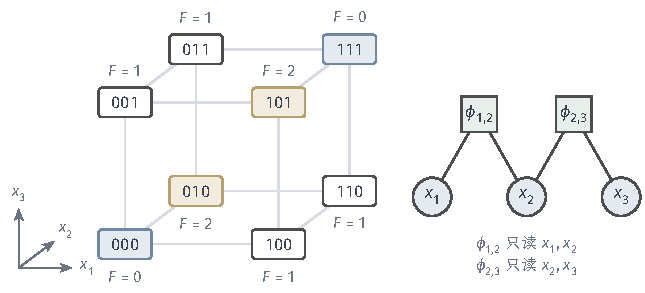
\includegraphics[width=109.269mm]{figures/01-basic-mathematics/04-graphs/tikz/c5-configuration-scopes/figure.pdf}
  \caption{配置空间与局部作用域。左：三个二值变量的$8$种配置排在立方体的顶点上，顶点旁的数是总成本$F=\phi_{1,2}+\phi_{2,3}$，其中相邻变量取值不同时成本为$1$；蓝色顶点成本为$0$，黄色顶点成本为$2$。右：圆点表示变量，方块表示局部函数，连线表示该函数读取的变量。每个局部函数只读取两个变量，但它们的和仍然对全部$8$种配置给出成本。}
  \label{fig:graph-dp-configuration-scopes}
\end{figure}

把这个例子一般化，设有一组局部项，用下标$a\in A$区分。每一项$\phi_a$只读取下标集合$S_a\subseteq V$中的变量，总成本为
\begin{equation}
F(\bm x)=\sum_{a\in A}\phi_a(\bm x_{S_a}),\qquad \bm x\in\mathcal X .
\label{eq:graph-dp-local-sum}
\end{equation}
这里的$\phi_a$称为\term{局部函数}（local function），也常称为\term{因子}（factor）；它读取的下标集合$S_a$称为$\phi_a$的\term{作用域}（scope）。“局部”限定的是读取范围：$\phi_a$精确地给出$\bm x_{S_a}$每种取值的成本，并不是对某个整体函数的近似；作用域也不限于两个变量，三元、四元的局部函数同样允许。一元项$\phi_i(x_i)$是作用域为$\{i\}$的特例。

局部函数的取值允许为$+\infty$，用来表示禁止的组合。例如设备$1,2$不能同时打开时，可以令$\phi_{1,2}(1,1)=+\infty$。约定$+\infty$加任何有限数或$+\infty$仍得$+\infty$，于是只要某一项禁止，整个配置的总成本就是$+\infty$。总成本有限的配置称为\term{可行配置}。这样，同一个式~\eqref{eq:graph-dp-local-sum}既表达偏好，也表达约束；求最小值时还要同时回答是否存在可行配置：最小值为$+\infty$，就说明所有配置都被某项禁止。

式~\eqref{eq:graph-dp-local-sum}是问题给出的分解，不是自动成立的性质。任意函数$F$都可以写成作用域为$V$的单个“局部”函数，但这时局部函数表就有$|\mathcal X|$项，与直接枚举没有区别。本章始终假定分解已经由问题给出，并且各作用域都较小；从一个任意给定的整体函数中寻找小作用域分解，是另一个问题。

\subsection{依赖图与因子图}

只有成对局部项时，可以用一个图记录哪些变量出现在同一项里：以变量为顶点，两个变量出现在同一个成对项中就连一条边。三台设备的例子得到路径$1-2-3$。这样的图记录的是函数的依赖关系，不是变量的取值本身；称“依赖结构是一条链”或“是一棵树”，指的就是这个图是路径或树。

三元及更高阶的局部项无法用一条边表示。这时把变量和局部函数分成两类节点：每个变量一个圆形节点，每个局部函数一个方形节点；变量属于某个局部函数的作用域时，在两者之间连边。这样得到的二部图称为\term{因子图}（factor graph）。因子图保留了每个局部函数的身份：两个不同的局部函数即使作用域相同，也是两个不同的方形节点。图~\ref{fig:graph-dp-configuration-scopes}右侧就是三台设备例子的因子图。

\paragraph{三种表示的对照}
考虑四个二值变量和两个三元局部函数，作用域分别为$S_A=\{1,2,3\}$和$S_B=\{2,3,4\}$。除因子图外，还有两种常用的结构表示。一种不保留函数节点，把每个作用域内的变量两两连边，得到的图称为\term{原始关系图}（primal graph），简称原始图。这里原始图有边$\{1,2\},\allowbreak\{1,3\},\allowbreak\{2,3\},\allowbreak\{2,4\},\allowbreak\{3,4\}$，唯独缺少$\{1,4\}$，因为变量$1$和$4$从不出现在同一个局部函数中。另一种允许一条“边”包含任意多个顶点：每个作用域记为一条\term{超边}（hyperedge），由此得到\term{超图}（hypergraph）。这里超图有两条超边$\{1,2,3\}$和$\{2,3,4\}$。图~\ref{fig:graph-dp-three-representations}并排画出了三种表示。

\begin{figure}[!htb]
  \centering
  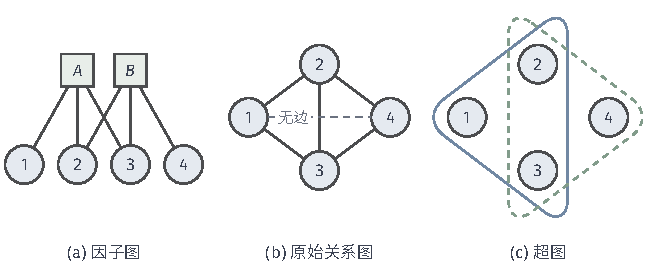
\includegraphics[width=111.936mm]{figures/01-basic-mathematics/04-graphs/tikz/c5-three-representations/figure.pdf}
  \caption{作用域$\{1,2,3\}$与$\{2,3,4\}$的三种结构表示。左：因子图，方块$A$、$B$是两个局部函数，连线表示读取关系。中：原始关系图，把每个作用域内的变量两两相连，只缺边$\{1,4\}$。右：超图，蓝色实线与绿色虚线围出的区域各是一条超边。若把两个三元函数换成五条边上的五个成对函数，原始图完全相同，而因子图和超图都会改变。}
  \label{fig:graph-dp-three-representations}
\end{figure}

原始图丢失了作用域的分组。若把$\phi_A,\phi_B$换成定义在五条边上的五个成对局部函数，原始图不变，因子图和超图却不同。更重要的是，相同的两两连接不能恢复函数表。设$\phi_A(x_1,x_2,x_3)$在$x_1+x_2+x_3$为偶数时取$0$、为奇数时取$+\infty$，$\phi_B$对$x_2+x_3+x_4$作同样的规定。$\phi_A$允许的取值恰为$(0,0,0),(0,1,1),(1,0,1),(1,1,0)$，其中任意两个变量的四种取值组合都出现过。因此，若只保留“每对变量允许哪些取值”的成对规则，这些规则什么也不禁止，$16$种配置都会被放行；而原问题中$x_2,x_3$确定后$x_1,x_4$都被唯一确定，只有$4$种可行配置。

超图保住了作用域的分组，但和原始图一样不保存局部函数的数值；因子图保住了函数身份，但仍需另外存储每个函数的取值表。后面的树分解以原始图为结构依据，因为原始图上的边已经足以说明哪些变量必须同时出现；计算时则始终使用完整的局部函数，不把它们拆成成对规则。

% 第5章第2节：链与树上的动态规划（链上的接口表递推、树上的消息与后序、最优配置的回溯）。

\section{链与树上的动态规划}
\label{sec:graph-tree-dp}

本节只考虑一元项和成对项，并假定成对项组成的依赖图没有环。这时总成本为
\begin{equation}
F(\bm x)=\sum_{i\in V}\phi_i(x_i)+\sum_{\{u,v\}\in E}\phi_{u,v}(x_u,x_v),
\label{eq:graph-dp-pairwise-cost}
\end{equation}
其中$\mathcal G=(V,E)$是依赖图，$\phi_{u,v}(x_u,x_v)$与$\phi_{v,u}(x_v,x_u)$指同一个局部函数。没有一元项的变量可以取$\phi_i\equiv0$。本节从链开始，说明怎样把已经处理过的变量压缩成一张只依赖接口变量的表；再把单个前驱推广为多个子树，得到树上的消息；最后说明怎样从这些表中恢复一个最优配置。依赖图带环、或者局部函数读取三个以上变量的情形，留到下一节。

\subsection{链上的递推}

\paragraph{固定接口变量}
先看三个变量的链$1-2-3$，每个变量取三档$\{0,1,2\}$，总成本$F=\phi_{1,2}(x_1,x_2)+\phi_{2,3}(x_2,x_3)$。两张局部函数表按行列给出：
\[
\bigl[\phi_{1,2}(x_1,x_2)\bigr]=\begin{bmatrix}4&1&3\\2&3&5\\3&4&2\end{bmatrix},\qquad
\bigl[\phi_{2,3}(x_2,x_3)\bigr]=\begin{bmatrix}1&3&2\\4&3&5\\2&2&4\end{bmatrix},
\]
左表的行对应$x_1=0,1,2$、列对应$x_2=0,1,2$，右表的行对应$x_2$、列对应$x_3$。直接枚举要计算$3^3=27$个配置的成本。

注意$x_1$只出现在$\phi_{1,2}$中。若先把$x_2$固定为某个值，$x_1$的选择就不再影响$\phi_{2,3}$，只需在左表的这一列中取最小。对$x_2=0,1,2$分别取列最小值，得到一张只依赖$x_2$的表
\[
m_{1\to2}(x_2)=\min_{x_1}\phi_{1,2}(x_1,x_2)=(2,\,1,\,2),
\]
达到最小值的$x_1$依次为$1,0,2$。这张表概括了链左端的全部信息：无论右侧怎样取值，只要$x_2$给定，左端最好的做法和它的成本都已确定。接下来只需在$x_2,x_3$上求
\[
\min_{x_2,x_3}\bigl[m_{1\to2}(x_2)+\phi_{2,3}(x_2,x_3)\bigr].
\]
对$x_2=0,1,2$，括号内对$x_3$的最小值依次为$2+1=3$、$1+3=4$、$2+2=4$，所以最优成本为$3$，在$x_2=0,x_3=0$时达到，再查表得$x_1=1$。整个过程计算了$9+9=18$个候选值，而不是$27$个配置；更重要的是，链越长，节省越多。

\paragraph{为什么可以这样分步}
这一步依据有限集合上最小值的三条规则。设$y,z$分别在有限集合中取值，$h$、$g$取值于$\mathbb R\cup\{+\infty\}$，$c$与$y$无关，则
\begin{equation}
\min_{y,z}h(y,z)=\min_{z}\min_{y}h(y,z),\qquad
\min_{y}\bigl[g(y)+c\bigr]=\min_{y}g(y)+c,
\label{eq:graph-dp-min-rules}
\end{equation}
并且对取值于互不相交变量组$y_1,\ldots,y_k$的函数，$\min_{y_1,\ldots,y_k}\sum_{r}g_r(y_r)=\sum_r\min_{y_r}g_r(y_r)$。第一条成立，因为两边都是同一个有限数集中的最小元；第二条成立，因为加上同一个$c$不改变比较结果；第三条成立，因为各$y_r$可以分别取到各自的最小点，而任何选择都不会使某一项小于它的最小值。$c$或某项为$+\infty$时，按$+\infty$加任何数仍为$+\infty$的约定，三条规则依然成立。把第一、二条用于三变量链，$\phi_{2,3}$对$x_1$而言是固定加项，于是$\min_{x_1}$可以移到$\phi_{1,2}$上。

\paragraph{一般链的递推}
现在设链为$1-2-\cdots-n$，总成本含一元项$\phi_k(x_k)$和相邻成对项$\phi_{k-1,k}(x_{k-1},x_k)$。记$D_k(x_k)$为前$k$个变量在$x_k$固定时的最小部分成本，即对$x_1,\ldots,x_{k-1}$求最小值后的
\[
\sum_{i=1}^{k}\phi_i(x_i)+\sum_{i=2}^{k}\phi_{i-1,i}(x_{i-1},x_i).
\]
固定$x_k$以后，前$k-1$个变量与$x_k$之间只有$\phi_{k-1,k}$一项联系，按式~\eqref{eq:graph-dp-min-rules}先对$x_1,\ldots,x_{k-2}$求最小值，再对$x_{k-1}$求最小值，得到
\begin{equation}
\begin{gathered}
D_1(x_1)=\phi_1(x_1),\\
D_k(x_k)=\phi_k(x_k)+\min_{x_{k-1}\in\mathcal X_{k-1}}\bigl[D_{k-1}(x_{k-1})+\phi_{k-1,k}(x_{k-1},x_k)\bigr],\quad k=2,\ldots,n,
\end{gathered}
\label{eq:graph-dp-chain-recursion}
\end{equation}
整条链的最小成本为$\min_{x_n}D_n(x_n)$。对$k$归纳即得递推的正确性：$D_{k-1}$已经是前$k-1$个变量的最小部分成本，而$\phi_k(x_k)$与$x_{k-1}$无关，可以移出最小化。这种把问题按顺序拆开、为每个子问题保存最优值表并由前一张表算出后一张表的做法称为\term{动态规划}（dynamic programming）。

\begin{algorithm}[链上的最小成本递推]
\label{alg:graph-dp-chain}
输入：链上各变量的有限状态集合、一元项表和相邻成对项表。输出：最小成本和一个最优配置。
\begin{enumerate}
  \item 令$D_1(x_1)=\phi_1(x_1)$。
  \item 对$k=2,\ldots,n$和每个$x_k$，计算式~\eqref{eq:graph-dp-chain-recursion}方括号中的全部候选值，取最小值记为$D_k(x_k)$，并把达到最小值的$x_{k-1}$（并列时取编号最小者）记为$p_k(x_k)$。
  \item 取使$D_n$最小的$x_n$；再对$k=n,\ldots,2$令$x_{k-1}=p_k(x_k)$。
\end{enumerate}
\end{algorithm}

\paragraph{二值链的逐轮表}
取$n=4$的二值链，一元项为$\phi_1=(0,3)$、$\phi_2=(2,0)$、$\phi_3=(3,0)$、$\phi_4=(1,2)$，括号内依次是取$0$和取$1$的成本；相邻成对项在两端取值相同时为$0$，不同时为$2$。按式~\eqref{eq:graph-dp-chain-recursion}，$D_1=(0,3)$；$D_2(0)=2+\min(0+0,3+2)=2$，$D_2(1)=0+\min(0+2,3+0)=2$，故$D_2=(2,2)$；同理$D_3=(3+\min(2,4),\,0+\min(4,2))=(5,2)$，$D_4=(1+\min(5,4),\,2+\min(7,2))=(5,4)$。图~\ref{fig:graph-dp-chain-recursion}画出了每一轮的表和每个候选中被选中的前驱。最小成本为$\min D_4=4$，在$x_4=1$处达到。

\begin{figure}[!htb]
  \centering
  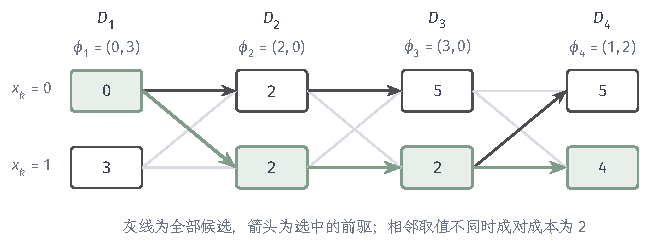
\includegraphics[width=109.587mm]{figures/01-basic-mathematics/04-graphs/tikz/c5-chain-recursion/figure.pdf}
  \caption{四变量二值链上的递推表。每列是一个变量，上下两格分别是$D_k(0)$与$D_k(1)$，列上方的小字为一元项。两列之间的灰色线表示全部候选，箭头从每个状态选中的前驱指向该状态，即回溯表$p_k$记录的选择。末列中$D_4(1)=4$最小，沿绿色箭头逆向读取得到最优配置$(0,1,1,1)$。逐点选取一元项最小的状态会得到$(0,1,1,0)$，成本为$5$。}
  \label{fig:graph-dp-chain-recursion}
\end{figure}

这个例子也说明了成对项的作用。若各变量只看自己的一元项，会选$(0,1,1,0)$：一元项合计为$1$，但两处取值变化要付$4$，总成本为$5$。递推得到的$(0,1,1,1)$在$x_4$上多付了$1$个单位的一元成本，却省掉了最后一处变化。

\paragraph{计算开销}
设每个变量至多有$q$个状态。每一轮要为$x_k$的每个状态比较至多$q$个候选，共至多$q^2$次候选计算，整条链约$nq^2$次。存储方面，每轮的$D_k$与回溯表$p_k$各至多$q$项，共约$2nq$项；若只要最优值而不恢复配置，任一时刻只需保留上一轮的表。与$q^n$次枚举相比，开销从指数降为线性于$n$。

\subsection{树上的递推}

\paragraph{从单个前驱到多个子树}
树没有链那样的天然顺序，但选定一个根$\rho$以后，每个非根顶点都有唯一的父点（第~\ref{sec:graph-trees-forests}节）。链上的$D_{k-1}$概括了$x_k$一侧的全部变量；在树上，一个顶点可能有多个子点，每个子点下面挂着一棵子树，需要分别概括后再合并。

对树的一条边$\{u,v\}$，删去它以后树分成两部分，记含$u$的那部分顶点集为$V_{u|v}$，称为$u$一侧。从$u$发往$v$的\term{消息}（message）是一张以$x_v$为索引的表，定义为
\begin{equation}
\begin{aligned}
m_{u\to v}(x_v)=\min_{x_u\in\mathcal X_u}\Bigl[&\phi_u(x_u)+\phi_{u,v}(x_u,x_v)\\
&+\sum_{r\in N(u)\setminus\{v\}}m_{r\to u}(x_u)\Bigr],
\end{aligned}
\label{eq:graph-dp-tree-message}
\end{equation}
其中$N(u)$是$u$在依赖图中的邻居集合。叶顶点只有一个邻居，求和为空，消息只由它自己的一元项和边上的成对项算出。下面的定理说明，这张表恰好概括了$u$一侧的全部成本。

\begin{theorem}[树上消息的含义]
\label{thm:graph-dp-tree-message}
设依赖图$\mathcal G=(V,E)$是有限树，总成本由式~\eqref{eq:graph-dp-pairwise-cost}给出。对任意边$\{u,v\}$，记$F_{u|v}$为$u$一侧的部分成本：$V_{u|v}$中各顶点的一元项、两端都在$V_{u|v}$中的成对项，再加上边$\{u,v\}$上的$\phi_{u,v}$。则对每个$x_v$，
\[
m_{u\to v}(x_v)=\min_{\bm x_{V_{u|v}}}F_{u|v}(\bm x_{V_{u|v}},x_v).
\]
进一步，对任意根$\rho$，$\min_{\bm x}F(\bm x)=\min_{x_\rho}\bigl[\phi_\rho(x_\rho)+\sum_{r\in N(\rho)}m_{r\to\rho}(x_\rho)\bigr]$。
\end{theorem}

\begin{proof}
对$|V_{u|v}|$归纳。删去$u$以后，$V_{u|v}\setminus\{u\}$按$u$的其他邻居$r\in N(u)\setminus\{v\}$分成互不相交的部分$V_{r|u}$。由树中路径的唯一性，不同部分之间没有边，否则会与$u$形成环。因此$F_{u|v}$可以拆成
\[
F_{u|v}=\phi_u(x_u)+\phi_{u,v}(x_u,x_v)+\sum_{r\in N(u)\setminus\{v\}}F_{r|u},
\]
其中每个$F_{r|u}$只依赖$x_u$与$\bm x_{V_{r|u}}$，并且每个局部项恰好出现在其中一处。固定$x_u$后，各$\bm x_{V_{r|u}}$是互不相交的变量组，由式~\eqref{eq:graph-dp-min-rules}后的第三条规则，对它们求最小值得到$\sum_r\min F_{r|u}$；由归纳假设，这个和等于$\sum_r m_{r\to u}(x_u)$。最后对$x_u$求最小值，就得到式~\eqref{eq:graph-dp-tree-message}。叶顶点是归纳的起点，此时求和为空，结论直接由定义得出。根处的等式用同样的拆分得到：$V\setminus\{\rho\}$按$\rho$的邻居分成互不相交的部分，每部分的最小成本是一条入消息。
\end{proof}

\paragraph{后序计算与分叉树算例}
式~\eqref{eq:graph-dp-tree-message}中，$u$发出消息前需要先收到来自其他邻居的消息。选定根后按后序处理顶点（先处理全部子点，再处理父点），每个顶点在收齐子点的消息后向父点发送一条消息，就满足了这个要求；最后在根处合并。图~\ref{fig:graph-dp-tree-messages}左半给出一个例子：树有边$\{1,3\},\allowbreak\{2,3\},\allowbreak\{3,4\},\allowbreak\{4,5\}$，以$3$为根；二值一元项为$\phi_1=(0,2)$、$\phi_2=(2,0)$、$\phi_3=(1,0)$、$\phi_4=(0,1)$、$\phi_5=(3,0)$；成对项在两端相同时为$0$，不同时分别为$1,1,2,1$（按上面边的顺序）。

后序为$1,2,5,4$。叶消息为$m_{1\to3}=(0,1)$，$m_{2\to3}=(1,0)$，$m_{5\to4}=(1,0)$，其中例如$m_{1\to3}(1)=\min(0+1,\,2+0)=1$。内部顶点$4$收到$m_{5\to4}$后向根发送
\[
\begin{aligned}
m_{4\to3}(x_3)&=\min_{x_4}\bigl[\phi_4(x_4)+\phi_{3,4}(x_3,x_4)+m_{5\to4}(x_4)\bigr]\\
&=\bigl(\min(0+0+1,\,1+2+0),\ \min(0+2+1,\,1+0+0)\bigr)=(1,1).
\end{aligned}
\]
根处合并一元项与三条入消息：$x_3=0$时为$1+0+1+1=3$，$x_3=1$时为$0+1+0+1=2$。因此最小总成本为$2$，根取$x_3=1$。整个计算只算了$4$条消息，每条消息比较$4$个候选，而枚举需要$2^5=32$个配置。

\begin{figure}[!htb]
  \centering
  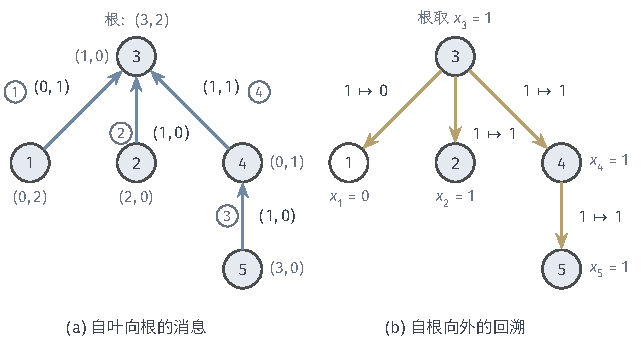
\includegraphics[width=108.514mm]{figures/01-basic-mathematics/04-graphs/tikz/c5-tree-messages/figure.pdf}
  \caption{分叉树上的消息与回溯。左：以$3$为根，按后序$1,2,5,4$发送消息；顶点旁的灰色二元组是一元项，箭头旁的二元组是消息表在接收端取$0$、$1$时的值，小圆圈中的序号是发送顺序；根合并后得到$(3,2)$。右：根取$x_3=1$后沿树向外查回溯表，黄色箭头旁的“$1\mapsto0$”表示父点取$1$时子点的最优选择为$0$；蓝色顶点取$1$，白色顶点取$0$，恢复的配置$(0,1,1,1,1)$成本为$2$。}
  \label{fig:graph-dp-tree-messages}
\end{figure}

\paragraph{每个顶点的最小成本表}
只求整体最优值时，一次自叶向根的计算已经足够。有时还需要知道每个顶点$v$取各个状态时整体能达到的最小成本，即$\min_{\bm x:\,x_v=s}F(\bm x)$。对根，这就是根处的合并结果；对其他顶点，还缺少来自父点一侧的消息。这时再按前序从根向叶发送一遍消息，同样使用式~\eqref{eq:graph-dp-tree-message}，然后在每个顶点合并全部入消息与一元项。仍以上例，从根发往$1$的消息为$m_{3\to1}=(2,1)$，于是$x_1$取$0$、$1$时的最小总成本为$(0+2,\,2+1)=(2,3)$，其最小值与整体最优值$2$一致。两遍计算共发送$2(n-1)$条消息；没有用到的方向不必计算。

\paragraph{计算开销}
每条消息对$x_v$的每个状态比较$x_u$的至多$q$个状态，每个候选要加上$|N(u)|$项，所以发出全部向上消息共需$O\bigl(\sum_u|N(u)|q^2\bigr)=O(nq^2)$次加法和比较，其中用到了树中$\sum_u|N(u)|=2(n-1)$。存储为$n-1$张消息表，每张至多$q$项。

\subsection{最优配置的回溯}

最优值只告诉我们最小成本是多少，并不直接给出达到它的配置。消息表经过了最小化，已经丢掉了“是哪一个$x_u$达到最小”的信息；若只保存最优值，事后只能重新枚举。解决办法是在计算每条消息时，为接收端的每个状态$x_v$同时记录达到最小值的$x_u$，组成一张\term{回溯表}$b_{u\to v}(x_v)$。并列最优时需要事先固定选择规则，本节约定取编号最小的状态。

\paragraph{从根向外读取}
回溯从根开始：取使根处合并值最小的$x_\rho$；然后按前序，对每个已确定取值的顶点$v$及其子点$u$，令$x_u=b_{u\to v}(x_v)$。由于每个子点只由父点的取值决定，这一过程沿树向外恰好给每个变量赋值一次。在图~\ref{fig:graph-dp-tree-messages}右半中，根取$x_3=1$；查表得$b_{1\to3}(1)=0$、$b_{2\to3}(1)=1$、$b_{4\to3}(1)=1$；再由$x_4=1$得$b_{5\to4}(1)=1$。恢复的配置为$(x_1,\ldots,x_5)=(0,1,1,1,1)$。

回溯得到的配置确实达到最优值。对子树大小归纳可知：若$x_v$已经确定，按回溯表给$u$一侧赋值后，$u$一侧的部分成本$F_{u|v}$恰好等于$m_{u\to v}(x_v)$，因为每一步选的$x_u$都达到式~\eqref{eq:graph-dp-tree-message}中的最小值，而子树内部又由归纳假设达到各条入消息的值。在根处合并后，总成本就等于根处的最小合并值。图~\ref{fig:graph-dp-chain-recursion}中的绿色箭头是链上的同一过程。

\paragraph{结果核对与不可行情形}
把恢复的配置代回全部原始局部项，可以独立核对结果。上例中一元项依次为$0,0,0,1,0$，合计$1$；成对项中只有边$\{1,3\}$两端不同，贡献$1$；总成本为$2$，与根处的值一致，而且每个局部项只计了一次。这样的核对不依赖消息计算本身，能发现表格或下标上的错误。

若根处的最小合并值为$+\infty$，说明每个配置都被某个局部项禁止，问题没有可行配置。这时应直接报告不可行，而不是把回溯得到的配置当作最优解输出，因为在全为$+\infty$的表中任何选择都“达到”最小值。另外，回溯表只恢复一个最优配置；若要列出全部并列最优的配置，需要在每个状态记录全部最优选择，而这类配置的数目本身可能随$n$指数增长。

% 第5章第3节：变量消元（消元操作与不变量、中间函数与填充边、消元次序与计算开销）。

\section{变量消元}
\label{sec:graph-variable-elimination}

链和树上的递推每次处理一个端点：把只连着已处理部分的变量汇总掉，留下一张接口表。一般依赖图可能有环，局部函数也可能读取三个以上变量，这时不一定存在只连着一个邻居的变量。本节把“汇总一个变量”写成对局部函数集合的一般操作，说明按任意次序逐个汇总都给出正确的最优值；随后会看到，正确性不依赖次序，中间表的大小却依赖次序。

本节沿用第~\ref{sec:graph-local-functions}节的四变量例子：二值变量$x_1,\ldots,x_4$，两个三元局部函数$\phi_A(x_1,x_2,x_3)$与$\phi_B(x_2,x_3,x_4)$，总成本$F=\phi_A+\phi_B$。两张表由表~\ref{tab:graph-dp-ternary-tables}给出，其中$+\infty$表示禁止的组合。

\begin{table}[!htb]
  \centering
  \caption{四变量例子的两个三元局部函数。第一列的三位二进制串对$\phi_A$表示$(x_1,x_2,x_3)$，对$\phi_B$表示$(x_2,x_3,x_4)$。}
  \label{tab:graph-dp-ternary-tables}
  \begin{tabular}{ccccccccc}
    \toprule
    取值 & $000$ & $001$ & $010$ & $011$ & $100$ & $101$ & $110$ & $111$\\
    \midrule
    $\phi_A(x_1,x_2,x_3)$ & $1$ & $0$ & $2$ & $+\infty$ & $0$ & $2$ & $1$ & $2$\\
    $\phi_B(x_2,x_3,x_4)$ & $2$ & $1$ & $0$ & $+\infty$ & $+\infty$ & $0$ & $1$ & $2$\\
    \bottomrule
  \end{tabular}
\end{table}

\subsection{消元操作}

\paragraph{汇总一个变量}
设当前有一组局部函数$\mathcal F$，总成本是它们的和。要汇总变量$x_i$，先找出所有作用域含$i$的函数，记为$\mathcal F_i$；它们的作用域之并去掉$i$，记为$R_i$。固定$R_i$中变量的取值后，把$\mathcal F_i$中的函数相加，再对$x_i$取最小，得到一个新函数
\begin{equation}
\psi_i(\bm x_{R_i})=\min_{x_i\in\mathcal X_i}\sum_{f\in\mathcal F_i}f .
\label{eq:graph-dp-elimination-step}
\end{equation}
然后从$\mathcal F$中删去$\mathcal F_i$，加入$\psi_i$；不含$i$的函数保持原样。这一操作称为消去$x_i$，逐个消去变量的方法称为\term{变量消元}（variable elimination）。链上的$m_{1\to2}$正是消去$x_1$时得到的新函数。

在四变量例子中消去$x_1$：只有$\phi_A$含$1$，$R_1=\{2,3\}$。对$(x_2,x_3)=(0,0),(0,1),(1,0),(1,1)$，分别比较$x_1=0,1$两行，得到
\[
\psi_1(x_2,x_3)=\bigl(\min(1,0),\ \min(0,2),\ \min(2,1),\ \min(+\infty,2)\bigr)=(0,\,0,\,1,\,2),
\]
达到最小值的$x_1$依次为$1,0,1,1$。消元后的函数集合是$\{\psi_1,\phi_B\}$。可以逐项核对它没有改变剩余变量的最优成本：例如取$(x_2,x_3,x_4)=(1,0,1)$，原问题对$x_1$求最小值为$\min\bigl(\phi_A(0,1,0)+\phi_B(1,0,1),\ \phi_A(1,1,0)+\phi_B(1,0,1)\bigr)=\min(2,1)=1$，新集合给出$\psi_1(1,0)+\phi_B(1,0,1)=1+0=1$，两者相同。

\paragraph{不变量与正确性}
上面的核对对每个剩余配置都成立，这不是巧合。设已经按某个次序消去了下标集合$Z$中的变量，把剩余变量的一个配置记为$\bm y=\bm x_{V\setminus Z}$。消元过程保持下面的不变量：
\begin{equation}
\sum_{f\in\mathcal F}f(\bm y)=\min_{\bm x_Z}F(\bm x_Z,\bm y)\qquad\text{对每个剩余配置}\ \bm y .
\label{eq:graph-dp-elimination-invariant}
\end{equation}

\begin{theorem}[变量消元的正确性]
\label{thm:graph-dp-elimination}
设各变量的状态集合有限，总成本由式~\eqref{eq:graph-dp-local-sum}给出。从$\mathcal F=\{\phi_a:a\in A\}$出发，按任意次序反复执行式~\eqref{eq:graph-dp-elimination-step}的消元操作，则每一步之后不变量~\eqref{eq:graph-dp-elimination-invariant}都成立。特别地，消去全部变量后剩下的常数（无变量的函数之和）等于$\min_{\bm x}F(\bm x)$；只消去$V\setminus Q$中的变量时，剩余函数之和是关于$\bm x_Q$的表，在每个$\bm x_Q$处等于$\min_{\bm x_{V\setminus Q}}F(\bm x)$。
\end{theorem}

\begin{proof}
开始时$Z=\varnothing$，当前函数之和就是$F$，不变量成立。设消去$x_i$之前不变量对$Z$成立。把当前函数分为含$i$的$\mathcal F_i$与其余部分$\mathcal F_{-i}$。固定$Z\cup\{i\}$以外的变量后，$\mathcal F_{-i}$中各函数的值与$x_i$无关，按式~\eqref{eq:graph-dp-min-rules}可以移出对$x_i$的最小化：
\[
\min_{x_i}\Bigl[\sum_{f\in\mathcal F_{-i}}f+\sum_{f\in\mathcal F_i}f\Bigr]
=\sum_{f\in\mathcal F_{-i}}f+\min_{x_i}\sum_{f\in\mathcal F_i}f
=\sum_{f\in\mathcal F_{-i}}f+\psi_i .
\]
右端正是消元后的函数之和。左端由不变量等于$\min_{x_i}\min_{\bm x_Z}F$，再由式~\eqref{eq:graph-dp-min-rules}的第一条等于$\min_{\bm x_{Z\cup\{i\}}}F$。所以不变量对$Z\cup\{i\}$成立。对消元步数归纳即得结论。
\end{proof}

\begin{algorithm}[变量消元求最小成本]
\label{alg:graph-dp-variable-elimination}
输入：有限状态集合、局部函数表、一个消元次序。输出：最小成本，以及（若需要）一个最优配置。
\begin{enumerate}
  \item 按次序取下一个变量$x_i$，找出当前全部含$i$的函数$\mathcal F_i$，确定$R_i$。
  \item 对$\bm x_{R_i}$的每个取值，枚举$x_i$的全部状态，按式~\eqref{eq:graph-dp-elimination-step}求$\psi_i$；同时把达到最小值的$x_i$（并列取编号最小者）记入回溯表$b_i(\bm x_{R_i})$。
  \item 用$\psi_i$替换$\mathcal F_i$，重复直到变量全部消去，剩下的常数即最小成本。
  \item 若最小成本有限，按消元的逆序依次令$x_i=b_i(\bm x_{R_i})$；由于$R_i$中的变量都比$x_i$晚消去，查表时它们已经取定。
\end{enumerate}
\end{algorithm}

逆序回溯的正确性与树上相同：每一步选的$x_i$达到式~\eqref{eq:graph-dp-elimination-step}的最小值，于是按逆序逐步代回不变量，恢复的配置使$F$等于最小成本。若只保存$\psi_i$而不保存回溯表，就无法恢复配置。

\subsection{中间函数与填充边}

消去一个变量时，新函数$\psi_i$的作用域$R_i$由所有含$i$的函数共同决定。在原始图上看，$R_i$恰好是$i$在当前原始图中的邻居集合：两个变量相邻，当且仅当它们同在某个当前函数的作用域中。新函数读取这些邻居的联合取值，所以消元后的原始图中，这些邻居两两相邻。

\paragraph{消去一个连着三个邻居的变量}
在四变量例子中改为先消去$x_2$。$\phi_A$与$\phi_B$都含$2$，$R_2=\{1,3\}\cup\{3,4\}=\{1,3,4\}$，新函数
\[
\psi_2(x_1,x_3,x_4)=\min_{x_2}\bigl[\phi_A(x_1,x_2,x_3)+\phi_B(x_2,x_3,x_4)\bigr]
\]
同时读取$x_1,x_3,x_4$。原始图中原来没有边$\{1,4\}$，消元后必须补上，如图~\ref{fig:graph-dp-elimination-step}所示。这样为记录新函数的联合依赖而补入的边称为\term{填充边}（fill-in edge）。填充边不表示原问题增加了约束：原来$x_1$与$x_4$通过$x_2$间接联系，消去$x_2$以后，这种间接联系只能由新函数直接记录。

\begin{figure}[!htb]
  \centering
  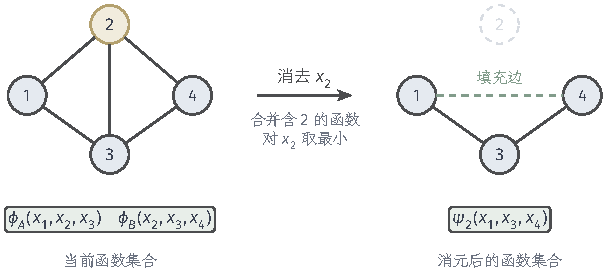
\includegraphics[width=102.687mm]{figures/01-basic-mathematics/04-graphs/tikz/c5-elimination-step/figure.pdf}
  \caption{消去$x_2$时的函数更新与图更新。左：消元前，黄色的$x_2$同时属于$\phi_A$与$\phi_B$的作用域，它的邻居是$1,3,4$。右：消元后，两个函数被新函数$\psi_2(x_1,x_3,x_4)$取代，$x_2$及其关联边被删除，邻居$1,3,4$两两相邻，其中绿色虚线$\{1,4\}$是填充边。}
  \label{fig:graph-dp-elimination-step}
\end{figure}

一般地，消元在原始图上对应一个纯粹的结构操作：把$i$的当前邻居两两连边，然后删去$i$及其关联边。不含$i$的函数提供的边保持不变；含$i$的函数在剩余变量之间提供的边都落在$R_i$内，已被补成的团覆盖。因此，消元后函数集合的原始图恰好是对原始图执行这一操作的结果。

\paragraph{数值计算与结构记账}
图上的操作只预测新函数可能同时读取哪些变量，不计算新函数的取值。对特殊的局部函数，新函数可能仍能进一步分解。例如，若$\phi_A(x_1,x_2,x_3)=g(x_1)+h(x_2,x_3)$，则
\[
\psi_2(x_1,x_3,x_4)=g(x_1)+\min_{x_2}\bigl[h(x_2,x_3)+\phi_B(x_2,x_3,x_4)\bigr],
\]
它是一个$x_1$的函数与一个$(x_3,x_4)$的函数之和，实际上并不需要同时索引$x_1$与$x_4$。图上的填充边不知道这种数值巧合，所以补边图给出的是通用情形下的作用域上界。后面讨论树分解时只使用这种结构记账：它适用于作用域给定、函数值任意的全部问题；具体函数是否还能化简，要回到数值表本身判断。

\subsection{消元次序与计算开销}

定理~\ref{thm:graph-dp-elimination}允许任意消元次序，不同次序给出相同的最优值，但中间函数的大小可以相差很多。下面在四变量例子上比较两个\term{消元次序}（elimination order）：$(1,4,2,3)$与$(2,1,3,4)$。

\paragraph{两种次序的逐步对照}
按$(1,4,2,3)$：消去$x_1$得到上面的$\psi_1(x_2,x_3)=(0,0,1,2)$；消去$x_4$时只有$\phi_B$含$4$，得到$\psi_4(x_2,x_3)=\min_{x_4}\phi_B=(1,0,0,1)$；消去$x_2$时合并$\psi_1,\psi_4$，得到只依赖$x_3$的表（记为$\psi_2'$，以区别于上面先消$x_2$时的$\psi_2$）$\psi_2'(x_3)=\bigl(\min(0+1,1+0),\ \min(0+0,2+1)\bigr)=(1,0)$；最后消去$x_3$得常数$0$。

按$(2,1,3,4)$消元时，第一步就要在$x_1,x_3,x_4$的$8$种取值下各比较$x_2$的两种状态，得到$8$项的$\psi_2$；其后得到的表依次为$(x_3,x_4)$上的$(2,1,0,4)$、$x_4$上的$(0,1)$，最后同样得常数$0$。表~\ref{tab:graph-dp-elimination-orders}列出了每一步的作用域和规模，图~\ref{fig:graph-dp-elimination-orders}画出了对应的图变化。

\begin{table}[!htb]
  \centering
  \caption{四变量例子上两种消元次序的逐步规模。“枚举”指计算新函数时要比较的候选组合数，即$R_i\cup\{i\}$上的配置数；“输出”指新函数表的项数，回溯表的项数与之相同。}
  \label{tab:graph-dp-elimination-orders}
  \begin{tabular}{cccccccc}
    \toprule
    \multicolumn{4}{c}{次序$(1,4,2,3)$} & \multicolumn{4}{c}{次序$(2,1,3,4)$}\\
    \cmidrule(lr){1-4}\cmidrule(lr){5-8}
    消去 & 新作用域 & 枚举 & 输出 & 消去 & 新作用域 & 枚举 & 输出\\
    \midrule
    $x_1$ & $\{2,3\}$ & $8$ & $4$ & $x_2$ & $\{1,3,4\}$ & $16$ & $8$\\
    $x_4$ & $\{2,3\}$ & $8$ & $4$ & $x_1$ & $\{3,4\}$ & $8$ & $4$\\
    $x_2$ & $\{3\}$ & $4$ & $2$ & $x_3$ & $\{4\}$ & $4$ & $2$\\
    $x_3$ & $\varnothing$ & $2$ & $1$ & $x_4$ & $\varnothing$ & $2$ & $1$\\
    \midrule
    合计 & & $22$ & $11$ & 合计 & & $30$ & $15$\\
    \bottomrule
  \end{tabular}
\end{table}

\begin{figure}[!htb]
  \centering
  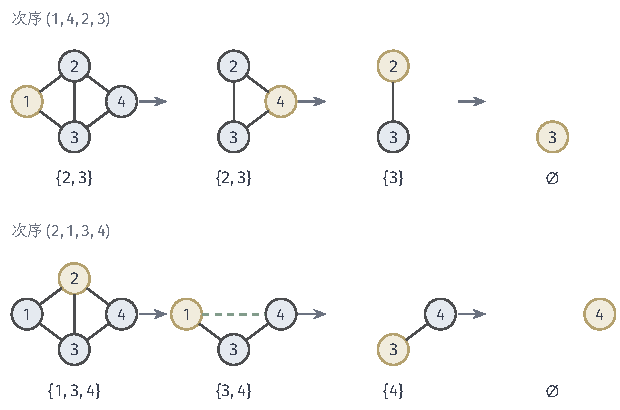
\includegraphics[width=105.004mm]{figures/01-basic-mathematics/04-graphs/tikz/c5-elimination-orders/figure.pdf}
  \caption{两种消元次序下原始图的变化。上行按$(1,4,2,3)$消元，每一步被消去的黄色顶点的邻居都已两两相邻，不产生填充边，新函数至多读取两个变量。下行按$(2,1,3,4)$消元，消去$2$时要补入填充边$\{1,4\}$（第二个图中的绿色虚线），新函数读取三个变量。每个图下方标出消去黄色顶点后新函数的作用域。}
  \label{fig:graph-dp-elimination-orders}
\end{figure}

两种次序都正确，也都恢复出同一个最优配置：$x_1=0$，$x_2=0$，$x_3=1$，$x_4=0$，代回表~\ref{tab:graph-dp-ternary-tables}得$\phi_A(0,0,1)+\phi_B(0,1,0)=0+0=0$。差别在于规模：第一种次序的最大中间表只有$4$项，第二种有$8$项。在这个小例子里差别不大；但若每个变量有$q$个状态，读取$r$个变量的表就有$q^r$项，多读取一个变量意味着表扩大$q$倍。

\paragraph{每一步的开销}
设消去$x_i$时$|R_i|=r_i$，各变量至多$q$个状态。计算$\psi_i$要对$R_i\cup\{i\}$的至多$q^{r_i+1}$种取值，各读取$\mathcal F_i$中每个函数一次，时间约为$|\mathcal F_i|\,q^{r_i+1}$；输出表与回溯表各至多$q^{r_i}$项。整个消元的时间由各步之和给出，主导项来自$r_i$最大的那一步。查找含$i$的函数还需要按变量维护的函数索引，这部分开销与函数个数成正比。

所以变量消元的规模取决于“最多同时处理多少个变量”，即$\max_i(r_i+1)$。这个数由依赖图和消元次序共同决定：有限状态并不保证精确消元总是可行，在某些图上，无论怎样排序，都会有一步需要同时处理很多变量。下一节用树分解描述这些同时处理的变量组，并用树宽给出与次序无关的结构度量。

% 第5章第4节：树分解与树宽（袋与接口、树分解的三个条件、团必被某袋容纳、宽度与树宽）。

\section{树分解与树宽}
\label{sec:graph-tree-decomposition}

上一节看到，变量消元的开销取决于每一步同时处理的变量组。本节把这些变量组单独拿出来，研究它们怎样组织成一棵树，才能让计算沿树进行而不丢失一致性。先从消元过程引出“袋”和“接口”，再给出合法分解的三个条件，最后用袋的大小定义宽度和树宽。本节只讨论结构本身：怎样构造分解放在第~\ref{sec:graph-tree-decomposition-construction}节，怎样在分解上计算放在第~\ref{sec:graph-bag-dp}节。

\subsection{袋与接口}

\paragraph{从消元步骤到袋}
回到四变量例子的次序$(1,4,2,3)$。消去$x_1$时要同时处理$\{1\}\cup R_1=\{1,2,3\}$，消去$x_4$时处理$\{2,3,4\}$，随后依次处理$\{2,3\}$和$\{3\}$。每一步产生的新函数会在后面某一步被用到：$\psi_1$与$\psi_4$都在消去$x_2$时被合并，$\psi_2'$在消去$x_3$时被使用。把每一步同时处理的变量集合看成一个节点，按“新函数交给哪一步使用”连接这些节点，就得到图~\ref{fig:graph-dp-bags-interface}中间的一棵树。

这种准备放进同一张表里同时索引的变量集合称为\term{袋}（bag），袋组成的树称为袋树。袋树的节点是计算单元，袋树的边表示两个计算单元之间传递一张表；它与原始图中连接两个变量的边含义不同。不同的袋可以有公共变量，例如$\{1,2,3\}$与$\{2,3,4\}$都含$2,3$。

\begin{figure}[!htb]
  \centering
  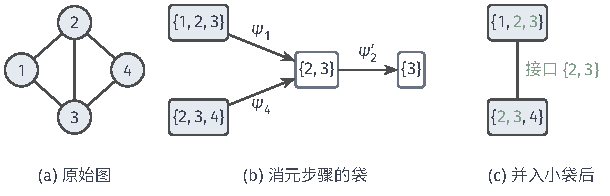
\includegraphics[width=103.283mm]{figures/01-basic-mathematics/04-graphs/tikz/c5-elimination-to-bags/figure.pdf}
  \caption{从消元步骤得到袋。左：四变量例子的原始图。中：按次序$(1,4,2,3)$消元时，每一步同时处理的变量集合构成一个袋，箭头表示新函数交给哪一步使用。右：$\{2,3\}$和$\{3\}$已包含在相邻的大袋中，并入后只剩两个袋，它们的交集$\{2,3\}$（绿色）就是接口。}
  \label{fig:graph-dp-bags-interface}
\end{figure}

袋与原始图中的“团”有关，但不必是团。原始图中两两相邻的顶点集合称为\term{团}（clique）。四变量例子中$\{1,2,3\}$是团，$\{1,2,4\}$不是，因为缺边$\{1,4\}$。按次序$(2,1,3,4)$消元时，第一步要同时处理$\{1,2,3,4\}$，这个袋在原始图中不是团，只在补入填充边后才成为团。所以袋可以重叠，也可以含有原图中不相邻的变量。

\paragraph{接口}
袋$\{2,3\}$和$\{3\}$都已包含在相邻的大袋中，可以并入，最后只剩两个袋$\{1,2,3\}$与$\{2,3,4\}$，如图~\ref{fig:graph-dp-bags-interface}右侧。相邻两袋的交集称为它们的接口（interface），这里是$\{2,3\}$。接口上的变量在两个袋里是同一个变量，不是两个副本：左袋在汇总$x_1$时必须对$(x_2,x_3)$的每种取值分别给出结果，右袋使用这些结果时也必须按同样的$(x_2,x_3)$取值来读。左袋的结果正是$\psi_1(x_2,x_3)$，一张以接口为索引的表。

由此提出一个要求。若某个变量出现在两个不相邻的袋中，而连接它们的袋树路径上有某个袋不含这个变量，那么两侧的计算无法通过接口约定这个变量取同一个值。为了让每个变量的取值在它出现的所有袋之间保持一致，袋的连接方式必须受到限制。下面把这个要求与覆盖要求一起写成定义。

\subsection{树分解的条件}

\paragraph{三个条件}
袋必须能容纳所有局部函数，袋之间的连接又必须保证一致。结构上，前一项要求每个变量和原始图的每条边都被某个袋包含，后一项就是上面提出的连接要求。

\begin{definition}[树分解]
\label{def:graph-dp-tree-decomposition}
设$\mathcal G=(V,E)$是有限无向图。$\mathcal G$的一个\term{树分解}（tree decomposition）由一棵有限树$\mathcal T$（节点集记为$T$）和每个节点$t\in T$上的子集$B_t\subseteq V$组成，满足：
\begin{enumerate}
  \item 顶点覆盖：每个顶点$v\in V$至少属于一个袋；
  \item 边覆盖：对每条边$\{u,v\}\in E$，存在某个袋同时含有$u$与$v$；
  \item 运行交集：对每个顶点$v\in V$，含$v$的节点集合$T_v=\{t\in T:v\in B_t\}$在$\mathcal T$中连通。
\end{enumerate}
第三个条件称为\term{运行交集性质}（running intersection property）。
\end{definition}

运行交集等价于：若$v$同时属于$B_s$和$B_t$，则$\mathcal T$中从$s$到$t$的路径上每个袋都含$v$。因为树中两点之间只有一条路径，$T_v$连通恰好意味着这条路径留在$T_v$中。

\paragraph{只覆盖边还不够}
图~\ref{fig:graph-dp-running-intersection}比较路径$1-2-3-4$上的两种袋连接。两种连接使用同样的三个袋$\{1,2\},\allowbreak\{2,3\},\allowbreak\{3,4\}$，都覆盖了全部顶点和边。上面一种按$\{1,2\}-\{2,3\}-\{3,4\}$连接，含$2$的两个袋相邻，含$3$的两个袋也相邻，是树分解。下面一种按$\{1,2\}-\{3,4\}-\{2,3\}$连接，含$2$的两个袋被不含$2$的袋$\{3,4\}$隔开。若沿这棵树计算，左端的袋可以选$x_2=0$，右端的袋可以选$x_2=1$，中间的袋不记录$x_2$，无从发现矛盾；拼起来的结果不对应任何一个配置。

\begin{figure}[!htb]
  \centering
  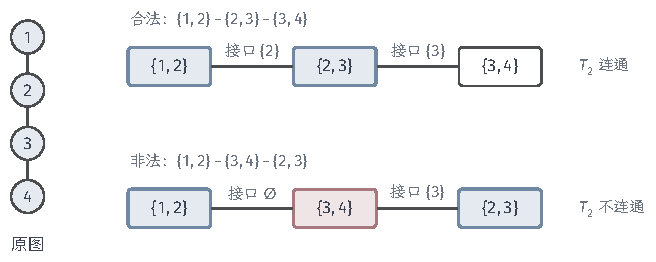
\includegraphics[width=111.016mm]{figures/01-basic-mathematics/04-graphs/tikz/c5-running-intersection/figure.pdf}
  \caption{路径$1-2-3-4$上的合法与非法袋连接。两种连接使用相同的三个袋，都覆盖全部顶点和边。上：含$2$的袋（蓝色）彼此相邻，含$3$的袋也相邻，满足运行交集。下：含$2$的两个袋之间隔着不含$2$的袋$\{3,4\}$（红色），$T_2$不连通，不是树分解。}
  \label{fig:graph-dp-running-intersection}
\end{figure}

\paragraph{完整作用域总能放进某个袋}
计算时每个局部函数要整个放进一个袋，因为袋表需要同时索引它的全部变量。一个作用域$S_a$在原始图上是团：其中任意两个变量同在$\phi_a$中，因而相邻。但树分解的定义只要求每条边被某个袋覆盖，三个变量两两成边时，三条边可能分别落在三个不同的袋中。下面的引理说明这种情况不会发生。

把每个顶点$v$的出现位置$T_v$看成袋树中的一棵连通子树。若$u,v$相邻，边覆盖给出一个同时含$u,v$的袋，于是$T_u$与$T_v$相交。对一个团$C$，各$T_v$（$v\in C$）两两相交；要证明的是它们有一个公共节点。

\begin{lemma}[团被某个袋容纳]
\label{lem:graph-dp-clique-in-bag}
设$(\mathcal T,\{B_t\}_{t\in T})$是$\mathcal G$的树分解，$C\subseteq V$是$\mathcal G$中的非空团，则存在节点$t\in T$使$C\subseteq B_t$。
\end{lemma}

\begin{proof}
任取袋树的一个节点作为根。对每个$v\in C$，$T_v$非空且连通。先说明$T_v$中有唯一一个离根最近的节点，记为$r_v$，并且$T_v$的每个节点都是$r_v$的后代（含$r_v$本身）。若$y\in T_v$不是$r_v$的后代，从$y$到$r_v$的树上路径要先向上经过$y$与$r_v$的最近公共祖先$z$，而$z$比$r_v$更靠近根；由$T_v$连通，这条路径留在$T_v$中，于是$z\in T_v$，与$r_v$的选取矛盾。同样的论证也说明离根最近的节点唯一。

在$C$中取一个顶点$w$，使$r_w$的深度在$\{r_v:v\in C\}$中最大。下面证明$r_w$属于每个$T_u$（$u\in C$）。$u=w$时，$r_w\in T_w$由定义成立。$u\neq w$时，$u,w$相邻，所以$T_u\cap T_w$中有某个节点$x$；$x\in T_w$，因而$x$是$r_w$的后代。考察$T_u$中从$x$到$r_u$的路径，它留在$T_u$中。若$r_u$不是$r_w$的后代，这条路径从$r_w$子树内部走到外部，必须经过$r_w$，于是$r_w\in T_u$。若$r_u$是$r_w$的后代，则$r_u$的深度不小于$r_w$的深度；而按$w$的选取，$r_u$的深度又不大于$r_w$的深度，所以$r_u=r_w$，同样有$r_w\in T_u$。因此$r_w$属于全部$T_u$，袋$B_{r_w}$含有整个$C$。
\end{proof}

图~\ref{fig:graph-dp-clique-in-bag}画出了证明中的几棵子树：每个变量的出现位置向上延伸到自己的最高节点，最高节点最深的那个变量，它的最高节点被其余各子树“经过”，因而就是要找的袋。

\begin{figure}[!htb]
  \centering
  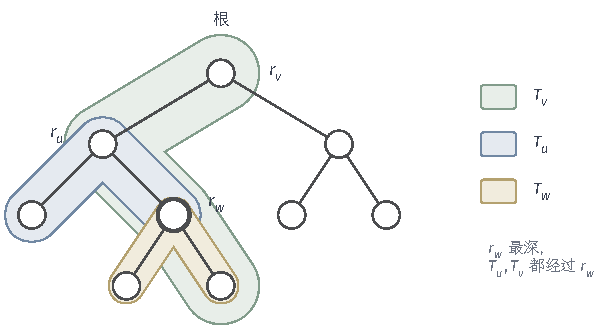
\includegraphics[width=102.648mm]{figures/01-basic-mathematics/04-graphs/tikz/c5-clique-in-bag/figure.pdf}
  \caption{团$\{u,v,w\}$被某个袋容纳的论证。袋树以顶部节点为根，三种颜色的区域分别是$T_u$、$T_v$、$T_w$，标签$r_u,r_v,r_w$标出各自离根最近的节点。$r_w$最深；$T_u$、$T_v$都要与$T_w$相交，而它们的最高节点不比$r_w$深，所以必须经过$r_w$。粗圈节点$r_w$的袋同时含$u,v,w$。}
  \label{fig:graph-dp-clique-in-bag}
\end{figure}

由引理~\ref{lem:graph-dp-clique-in-bag}，原始图的任一树分解中，每个局部函数的完整作用域都被某个袋整体容纳。因此在原始图上构造树分解就足够了，不需要额外记录高阶作用域；第~\ref{sec:graph-local-functions}节所说的“结构以原始图为依据、计算保留完整函数”在这里得到保证。

\subsection{宽度与树宽}

袋越大，袋表越大。为了用一个数概括一次分解的规模，定义树分解的宽度为$\max_{t\in T}|B_t|-1$，即最大袋的大小减一；图$\mathcal G$的\term{树宽}（treewidth）是它的全部树分解宽度的最小值，记为$\operatorname{tw}(\mathcal G)$。减一是一种约定，使得下面的树恰好宽度为一。

\paragraph{三个小例子}
单个顶点的图只需一个袋$\{1\}$，宽度为$0$，任何没有边的图都如此。至少含一条边的树宽度为$1$：任选根$\rho$，为每个非根顶点$u$建袋$\{u,p(u)\}$，其中$p(u)$是父点；若$p(u)$不是根，就把这个袋连到$p(u)$自己的袋上，根的各子点的袋则依次连成一条链。这样，非根顶点$v$出现在自己的袋和各子点的袋中，后者都与前者相邻；根只出现在各子点的袋中，它们连成链，所以运行交集成立。另一方面，一条边要求某个袋含两个顶点，宽度不能小于$1$。

四个顶点的环$1-2-3-4-1$有宽度为$2$的树分解：两个袋$\{1,2,3\}$与$\{1,3,4\}$，以一条边相连，接口为$\{1,3\}$。它没有宽度为$1$的树分解。证明沿用引理~\ref{lem:graph-dp-clique-in-bag}的思路：给任一树分解选根，在环上取$w$使$r_w$最深，$w$在环上的两个邻居$u,v$各自与$w$相邻，于是$T_u$、$T_v$都与$T_w$相交，上面的论证表明$r_w\in T_u\cap T_v$。这个袋含$u,v,w$三个顶点，所以宽度至少为$2$。这一论证对任何环都适用：含环的图树宽至少为$2$，树宽为$1$的图恰好是至少含一条边的森林（森林的各个分量分别按上面的方法分解，再用任意的边把各分量的袋树连成一棵树；不同分量没有公共顶点，这些连接不影响运行交集）。

这几个例子说明，树宽衡量的是图与树的接近程度：一条边需要两个变量同时出现，一个环则迫使某处至少三个变量同时出现。还要注意，某一次构造得到宽度$k$，只说明$\operatorname{tw}(\mathcal G)\leq k$；要断言树宽恰为$k$，还需要像上面那样证明不存在更小宽度的分解。

\paragraph{宽度与表的大小}
若每个变量至多有$q$个状态，宽度为$k$的分解中，每个袋至多有$k+1$个变量，稠密存储的袋表至多$q^{k+1}$项。这是第~\ref{sec:graph-bag-dp}节中主要的枚举规模。实际的总开销还包括袋的个数、接口的大小和每次读取局部函数的成本，宽度只控制其中随状态数指数增长的那一部分。

最后，寻找树宽最小的分解与使用一个已经给定的分解是两项不同的任务。前者在一般图上是困难的组合问题；后者只需检查三个条件并沿树计算。第~\ref{sec:graph-tree-decomposition-construction}节给出的构造方法都只保证得到合法的分解和宽度上界。

% 第5章第5节：树分解的构造（由消元次序构造、最小度与最小填充、弦图与完美消元序、团树与最大权生成树）。

\section{树分解的构造}
\label{sec:graph-tree-decomposition-construction}

上一节给出了树分解的合法性条件，但没有说明怎样得到一个分解。本节先说明，任何一个完整的消元次序都能机械地产生一个树分解，其宽度就是该次序下最大的中间作用域；再讨论没有给定次序时怎样选择次序。最后考虑一类不需要补边的图，即弦图，在其上可以直接用极大团作袋，并用第~\ref{sec:graph-minimum-spanning-tree}节的最大权生成树把它们连成团树。与第~\ref{sec:graph-variable-elimination}节不同，本节只做结构上的操作：输出袋和袋之间的连接，不计算任何成本表。

\subsection{基于消元次序的构造}

\paragraph{逐轮记录袋}
输入非空有限无向图$\mathcal G=(V,E)$和一个包含每个顶点恰好一次的消元次序$\pi$。按$\pi$逐个处理顶点：处理$v$时，读出$v$在当前图中的邻居集合，记为$N^+_\pi(v)$（上标$+$表示这些邻居都在次序中排在$v$之后）；记录袋$B_v=\{v\}\cup N^+_\pi(v)$；把$N^+_\pi(v)$中的顶点两两连边，然后删去$v$及其关联边。这正是第~\ref{sec:graph-variable-elimination}节中消元在原始图上的结构操作，袋$B_v$就是消去$x_v$时同时处理的变量组。

关键在于每一轮都要从更新后的图读取邻居。图~\ref{fig:graph-dp-elimination-to-decomposition}的例子有边$\{1,2\},\allowbreak\{1,4\},\allowbreak\{2,3\},\allowbreak\{3,4\},\allowbreak\{3,5\},\allowbreak\{4,5\}$，次序为$(1,2,5,3,4)$。处理$1$时，邻居$2,4$不相邻，补入填充边$\{2,4\}$，记袋$\{1,2,4\}$。处理$2$时，当前邻居是$\{3,4\}$，其中$4$是刚补入的邻居，记袋$\{2,3,4\}$。若误从原图读取，$2$的剩余邻居只有$3$，袋$\{2,3\}$就漏掉了消去$x_1$后新函数同时读取的$x_2,x_4$。随后依次记袋$\{3,4,5\}$、$\{3,4\}$、$\{4\}$，不再需要补边。

\paragraph{连接父袋}
袋记录完毕后，对每个$N^+_\pi(v)$非空的顶点$v$，令$p(v)$为$N^+_\pi(v)$中在次序里最早的顶点，把$B_v$连到$B_{p(v)}$；$N^+_\pi(v)$为空的袋没有父袋，作为根。原图不连通时会有多个根，可以再用任意边把这些根连成一棵树，这些边的接口为空。在上例中$p(1)=2$、$p(2)=3$、$p(5)=3$、$p(3)=4$，得到以$B_4=\{4\}$为根的袋树，最大袋含$3$个顶点，宽度为$2$。

\begin{figure}[!htb]
  \centering
  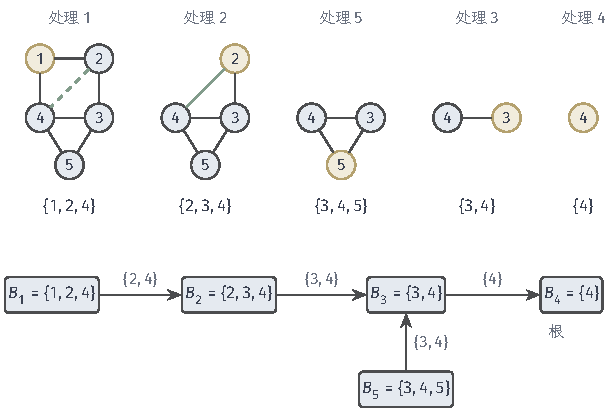
\includegraphics[width=104.369mm]{figures/01-basic-mathematics/04-graphs/tikz/c5-elimination-to-decomposition/figure.pdf}
  \caption{由消元次序$(1,2,5,3,4)$构造树分解。上行：每一轮的当前图，黄色为正在处理的顶点，绿色虚线为本轮补入的填充边，下一轮中它以绿色实线留在当前图里；图下标出记录的袋。下：按“连到最早被处理的后续邻居”连接父袋得到的袋树，箭头指向父袋，边旁标出接口。}
  \label{fig:graph-dp-elimination-to-decomposition}
\end{figure}

下面的定理说明这样得到的结构总是树分解。消元次序$\pi$下的最大后续邻居数$\max_v|N^+_\pi(v)|$称为$\pi$的\term{诱导宽度}（induced width）。

\begin{theorem}[消元次序产生树分解]
\label{thm:graph-dp-elimination-decomposition}
设$\mathcal G$是非空有限无向图，$\pi$是它的完整消元次序。按上面的方法记录袋$B_v=\{v\}\cup N^+_\pi(v)$并连接父袋（多个根之间用空接口边连接），得到的是$\mathcal G$的树分解，其宽度等于$\pi$的诱导宽度。因此$\mathcal G$的树宽不超过任何消元次序的诱导宽度。
\end{theorem}

\begin{proof}
先说明袋树是树。每个非根袋恰有一条通向父袋的边，而父点$p(v)$在次序中排在$v$之后，沿父边前进时次序位置严格增大，所以不会回到出发点，不形成环。每条父链都在有限步后到达一个根，各根之间再用树边连接，整体连通且无环。

顶点覆盖由$v\in B_v$给出。边覆盖：设$\{u,v\}\in E$且$u$先于$v$被处理。在处理$u$之前，图中只删去过已处理的顶点及其关联边，所以边$\{u,v\}$仍在，$v\in N^+_\pi(u)$，于是$B_u$同时含$u,v$。

运行交集：设$z\in B_v$且$v\neq z$，只需证明从$B_v$沿父链向上的每个袋都含$z$，直到到达$B_z$；这样含$z$的每个袋都与$B_z$由一条全部含$z$的路径相连，$T_z$连通。由于$z\in N^+_\pi(v)$，父点$p(v)$要么就是$z$，要么排在$z$之前。若$p(v)\neq z$，处理$v$时$z$与$p(v)$都是$v$的邻居，补团操作使它们相邻；在处理$p(v)$之前$z$没有被删除，这条边仍在，所以$z\in N^+_\pi(p(v))\subseteq B_{p(v)}$。对$p(v)$重复同样的论证，次序位置严格增大，最终到达$B_z$。

宽度为$\max_v|B_v|-1=\max_v|N^+_\pi(v)|$，即诱导宽度。树宽是全部树分解宽度的最小值，所以不超过它。
\end{proof}

证明中的边覆盖论证同样适用于填充边，因此所得袋树也是补边后图的树分解。构造的结构开销可以分开报告：设处理第$t$个顶点时它有$d_t$个当前邻居，补边要检查$\sum_t d_t(d_t-1)/2$对顶点，记录的袋共含$\sum_t(d_t+1)$个顶点；用支持常数时间查边和加边的邻接集合实现时，时间为$O\bigl(n+m+\sum_t d_t^2\bigr)$。这只是结构操作的开销；第~\ref{sec:graph-bag-dp}节在袋上计算成本表时，开销随袋大小指数增长，需要另算。

\subsection{消元次序的选择}

定理~\ref{thm:graph-dp-elimination-decomposition}把找好的树分解归结为找诱导宽度小的消元次序。在一般图上找最优次序是困难的，实践中常用局部规则每轮挑选一个顶点。两条常见规则是：\term{最小度启发式}（min-degree），选当前邻居最少的顶点；\term{最小填充启发式}（min-fill），选消去时需要补边最少的顶点，即当前邻域中缺少的边数最少者。

\begin{algorithm}[贪心选择消元次序]
\label{alg:graph-dp-greedy-order}
输入：非空有限无向图和一条评分规则（当前度数或当前缺边数）。输出：消元次序、各轮的袋和填充边。
\begin{enumerate}
  \item 对当前图中的每个顶点按规则计算评分，取评分最小者，评分相同时取编号最小者，记为$v$。
  \item 记录袋$\{v\}\cup N(v)$，把$N(v)$补成团，删去$v$，并把$v$追加到次序末尾。
  \item 若图非空，回到第1步，并在更新后的图上重新计算评分。
\end{enumerate}
\end{algorithm}

评分必须在每轮更新后的图上重算。若只按初始度数排一次序，或用原图的缺边数代替当前缺边数，得到的就不是这两条规则，因为补边会改变其他顶点的度数和邻域。

\paragraph{同一图上的两种评分}
图~\ref{fig:graph-dp-min-degree-min-fill}的图有六个顶点和边$\{1,3\},\allowbreak\{1,4\},\allowbreak\{1,5\},\allowbreak\{1,6\},\allowbreak\{2,3\},\allowbreak\{2,4\},\allowbreak\{2,6\},\allowbreak\{3,5\},\allowbreak\{4,5\},\allowbreak\{5,6\}$。初始度数依次为$4,3,3,3,4,3$；缺边数依次为$3,3,2,2,3,2$，例如顶点$2$的邻居$3,4,6$两两不相邻，缺$3$条边，而顶点$3$的邻居$1,2,5$中只缺$\{1,2\}$与$\{2,5\}$。最小度规则在度数为$3$的$2,3,4,6$中按编号选$2$，补入$\{3,4\},\allowbreak\{3,6\},\allowbreak\{4,6\}$；此后剩下的五个顶点度数都是$4$，选$1$时袋为$\{1,3,4,5,6\}$，宽度升到$4$。最小填充规则先选缺边最少的$3$，补入两条边，袋为$\{1,2,3,5\}$；其后依次选$4,1,2,5,6$，不再补边，最大袋含$4$个顶点，宽度为$3$。

\begin{figure}[!htb]
  \centering
  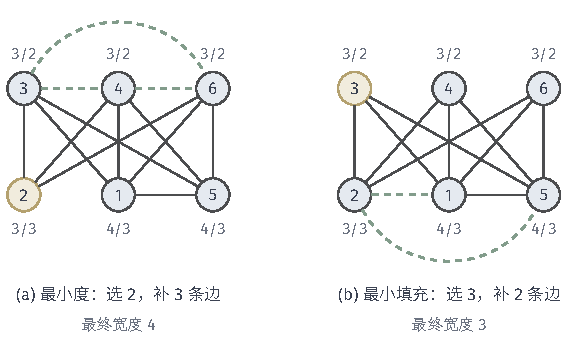
\includegraphics[width=96.778mm]{figures/01-basic-mathematics/04-graphs/tikz/c5-min-degree-min-fill/figure.pdf}
  \caption{最小度规则与最小填充规则的第一步。每个顶点旁的“$d/f$”是当前度数与当前缺边数。左：最小度规则在度数为$3$的顶点中按编号选$2$（黄色），要补三条绿色虚线，最终宽度为$4$。右：最小填充规则选缺边最少的$3$（黄色），只补两条边，最终宽度为$3$。}
  \label{fig:graph-dp-min-degree-min-fill}
\end{figure}

\paragraph{启发式只给出上界}
两种规则都只看一步：度数小不代表补边少，补边少也不保证以后的袋小。上例中最小度规则受平局规则影响，得到的宽度比最小填充多$1$；穷举全部$720$个消元次序可以核对，这个图上任何次序的诱导宽度都不小于$3$，所以最小填充在这里恰好达到了最好的次序。但换一个图，最小填充同样可能不是最优。因此报告结果时应分开写出构造的宽度、填充边数和结构操作次数，并把宽度理解为树宽的上界，而不是树宽本身。按算法~\ref{alg:graph-dp-greedy-order}的直接实现，每轮要为全部剩余顶点重算评分，最小填充一轮的检查量可达$\sum_v|N(v)|^2$；若用缓存只更新受补边影响的顶点，需要说明哪些边的增删会触发重算。

\subsection{弦图上的无填充消元}

\paragraph{单纯顶点与完美消元序}
填充边会使袋变大，最理想的情形是全程不需要补边。处理顶点$v$时不需要补边，当且仅当$v$的当前邻居已经两两相邻。当前邻居构成团的顶点称为\term{单纯顶点}（simplicial vertex）；没有邻居或只有一个邻居的顶点也算单纯顶点。若一个消元次序使每个顶点在被处理时都是当前图中的单纯顶点，就称它为\term{完美消元序}（perfect elimination ordering）。沿完美消元序消元不产生任何填充边，当前图始终是原图在剩余顶点上的诱导子图。

\paragraph{弦与弦图}
不是每个图都有完美消元序。四个顶点的环$1-2-3-4-1$中，每个顶点的两个邻居都不相邻：$1$与$3$的邻居都是$\{2,4\}$，缺边$\{2,4\}$；$2$与$4$的邻居都是$\{1,3\}$，缺边$\{1,3\}$。所以第一步就找不到单纯顶点。补入边$\{1,3\}$后，顶点$2$的邻居$\{1,3\}$相邻，可以先消去；剩下的三角形$1,3,4$中每个顶点都单纯，于是$(2,1,3,4)$是完美消元序。图~\ref{fig:graph-dp-chordal-four-cycle}画出了这一对比。

\begin{figure}[!htb]
  \centering
  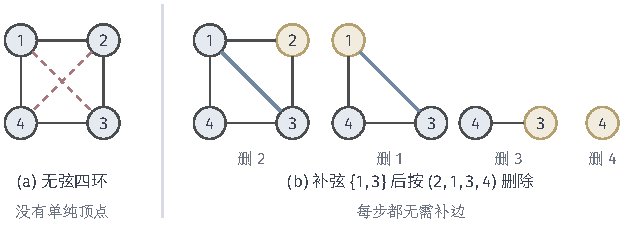
\includegraphics[width=106.306mm]{figures/01-basic-mathematics/04-graphs/tikz/c5-chordal-four-cycle/figure.pdf}
  \caption{无弦四环与补弦后的图。左：四环中每个顶点的两个邻居都不相邻（红色虚线为所缺的边），没有单纯顶点。右：补入弦$\{1,3\}$（蓝色）后，按$(2,1,3,4)$逐个删除，每一步被删除的黄色顶点的剩余邻居都已相邻，全程无填充。}
  \label{fig:graph-dp-chordal-four-cycle}
\end{figure}

四环的问题出在“长度至少为四而没有捷径的环”。在长度至少为$4$的环上，连接两个在环上不相邻的顶点的边称为该环的\term{弦}（chord）。每个长度至少为$4$的环都有弦的有限无向图称为\term{弦图}（chordal graph）。树没有环，是弦图；补入$\{1,3\}$后的四环是弦图；无弦四环不是。给一般图补边使之成为弦图称为\term{弦化}（chordal completion）。任何消元次序补边后的图都是弦图，因为该次序就是补边后图的完美消元序，由下面的定理即知；所以第一小节的构造实际上隐含了一次弦化。

\begin{theorem}[弦图与完美消元序]
\label{thm:graph-dp-chordal-peo}
有限无向图是弦图，当且仅当它有完美消元序。
\end{theorem}

\begin{proof}
先证有完美消元序的图是弦图。设图中有长度至少为$4$且无弦的环，考察环上最先被处理的顶点$v$。$v$在环上的两个邻居$u,w$此时都还在图中，并且与$v$相邻。$v$是单纯顶点，所以$u,w$相邻；而沿完美消元序处理时从不补边，$\{u,w\}$必是原图的边。环长至少为$4$，$u,w$在环上不相邻，于是$\{u,w\}$是这个环的弦，矛盾。

反方向的论证路线如下。第一步是一个引理：每个非空有限弦图都有单纯顶点，若它不是完全图，还有两个不相邻的单纯顶点。这一步需要分析极小分隔集，证明极小分隔集在弦图中都是团，本书不展开。第二步，弦图的诱导子图仍是弦图，因为诱导子图中的无弦环在原图中也无弦。于是可以反复删去一个单纯顶点，余下的图仍是弦图、仍有单纯顶点，直到删完，删除的次序就是完美消元序。
\end{proof}

\paragraph{构造与核验}
定理只说明弦图有完美消元序，并没有给出高效的求法。最直接的构造是逐次寻找单纯顶点：在当前图中按编号检查每个顶点，枚举它的每对邻居看是否相邻，找到第一个单纯顶点就删去它并追加到次序中；若非空的当前图中找不到单纯顶点，就报告输入不是弦图，并返回这个当前图作为证据，而不暗中补边。每轮最多检查$n$个顶点，检查顶点$v$需要$O(|N(v)|^2)$次查边，直接实现的总检查量最坏可达$O(n^4)$。存在线性时间的专门算法，这里不展开。

构造得到的次序应当独立核验。给定原图和一个次序，先确认它恰好包含每个顶点一次，再为每个顶点记下次序位置；对每个$v$取出原图中排在它之后的邻居，检查它们是否两两相邻。全部通过时次序是完美消元序，因为在不补边的前提下，处理$v$时的当前邻居恰好就是这些后续邻居；发现缺边时，就把$v$和那对不相邻的邻居作为失败证据返回。核验的检查量为$O(n+m)$再加$\sum_v|N^+_\pi(v)|^2$次查边。例如把$(2,1,3,4)$用于无弦四环，第一个顶点$2$的后续邻居$\{1,3\}$不相邻，立即被拒绝；用于补弦后的图则通过。

\paragraph{极大团与最大团}
弦图上可以直接用团作袋，这需要区分两种“最大”。不能再加入任何其他顶点而保持两两相邻的团称为\term{极大团}（maximal clique），这是按集合包含判断的；在所有团中顶点数最多的称为\term{最大团}（maximum clique）。例如三角形$1,2,3$外加一条边$\{3,4\}$，极大团是$\{1,2,3\}$和$\{3,4\}$；后者不能再扩大，但只有两个顶点，不是最大团。下面的团树需要全部极大团，而不只是最大的几个。

\subsection{团树的构造}

以弦图的全部极大团为袋、并满足运行交集的树分解称为\term{团树}（junction tree，也称clique tree）。团树中每个袋都是团，没有因填充而多出的变量，相邻两袋的交集就是它们共享的变量。本小节回答两个问题：怎样从完美消元序得到全部极大团；怎样把它们连成满足运行交集的树。

\paragraph{从完美消元序得到极大团}
设$\pi$是已经核验的完美消元序。对每个顶点$v$，候选集合$K_v=\{v\}\cup N^+_\pi(v)$是团，因为$v$被处理时是单纯顶点。反过来，任一团$C$都包含在某个$K_v$中：取$C$中最先被处理的顶点$v$，$C$的其余顶点都在$v$之后且与$v$相邻，所以都属于$N^+_\pi(v)$。因此极大团恰好是候选集合中不被其他候选严格包含的那些。具体做法是：生成全部$K_v$，删去重复的集合，再删去被其他候选严格包含的集合。

图~\ref{fig:graph-dp-clique-tree-mst}的弦图有边$\{1,2\},\allowbreak\{1,3\},\allowbreak\{2,3\},\allowbreak\{2,4\},\allowbreak\{3,4\},\allowbreak\{3,5\},\allowbreak\{4,5\}$，$(1,2,5,3,4)$是它的完美消元序。候选集合为$K_1=\{1,2,3\}$、$K_2=\{2,3,4\}$、$K_5=\{3,4,5\}$、$K_3=\{3,4\}$、$K_4=\{4\}$；删去被包含的$K_3,K_4$，得到三个极大团$A=\{1,2,3\}$、$B=\{2,3,4\}$、$C=\{3,4,5\}$。

\paragraph{用最大权生成树连接}
直觉上，共享变量多的团应该相邻，这样接口才能携带足够的共同变量。在以极大团为顶点的完全图上，给每对团$C,D$赋权$w(C,D)=|C\cap D|$，交集为空的零权边也保留；然后求这个图的最大权生成树，可以把权取负后调用第~\ref{sec:graph-minimum-spanning-tree}节的Kruskal或Prim方法。上例中$w(A,B)=2$、$w(B,C)=2$、$w(A,C)=1$，最大权生成树是$A-B-C$，总权为$4$。若改选$A-B$与$A-C$，总权为$3$，此时含$4$的两个团$B,C$之间隔着不含$4$的$A$，运行交集被破坏，如图~\ref{fig:graph-dp-clique-tree-mst}右侧所示。

\begin{figure}[!htb]
  \centering
  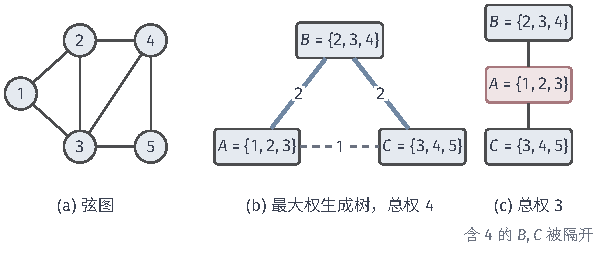
\includegraphics[width=102.306mm]{figures/01-basic-mathematics/04-graphs/tikz/c5-clique-tree-mst/figure.pdf}
  \caption{用交集权重的最大权生成树连接极大团。左：弦图。中：三个极大团组成的候选完全图，边上的数是交集大小，蓝色粗线是总权为$4$的最大权生成树$A-B-C$，虚线是未被选中的候选边。右：总权为$3$的另一棵生成树$B-A-C$，含$4$的团$B,C$被不含$4$的$A$（红色）隔开，不满足运行交集。}
  \label{fig:graph-dp-clique-tree-mst}
\end{figure}

下面的定理说明，这个例子中的对应关系是一般的。

\begin{theorem}[团树与最大权生成树]
\label{thm:graph-dp-clique-tree-mst}
设$\mathcal H$是非空有限弦图，$\mathcal C$是它的全部极大团。在以$\mathcal C$为顶点的完全图上令$w(C,D)=|C\cap D|$。则一棵生成树满足运行交集，当且仅当它的总权最大。
\end{theorem}

\begin{proof}
先给出任意生成树的总权上界。对生成树$\mathcal T'$，把每条边的权按共享变量拆开计数：
\[
\sum_{\{C,D\}\in\mathcal T'}|C\cap D|=\sum_{v}e_v,
\]
其中$e_v$是两端都含$v$的树边条数。设$v$属于$r_v$个极大团，两端都含$v$的树边正是$\mathcal T'$在这$r_v$个节点上的诱导子图的边；树的诱导子图没有环，是$r_v$个节点上的森林，所以$e_v\leq r_v-1$，且等号成立当且仅当这个诱导子图连通，即含$v$的团在$\mathcal T'$中连通。于是总权不超过$\sum_v(r_v-1)$，等号成立当且仅当对每个$v$都满足运行交集。

剩下要证明确实存在满足运行交集的生成树，即团树存在；那时最大总权恰为$\sum_v(r_v-1)$，最大权生成树就是满足运行交集的生成树。取一个完美消元序，按定理~\ref{thm:graph-dp-elimination-decomposition}的方法以$K_v$为袋得到树分解。若某个袋包含于相邻的袋，就把这条袋树边收缩，只保留较大的袋：顶点覆盖和边覆盖不受影响；对运行交集，被收缩的较小袋中的变量都在较大袋中，收缩一条两端都含$v$的边不破坏$T_v$的连通性，而不含$v$的较小袋本来不在$T_v$中，收缩后$T_v$也不变。反复收缩，直到没有相邻两袋有包含关系。这时任何两个袋都没有包含关系：若$B_s\subseteq B_t$而$s,t$不相邻，取路径上与$s$相邻的节点$s'$，由运行交集$B_s$的每个变量都在$B_{s'}$中，与“相邻袋无包含关系”矛盾。各袋都是团且互不包含；每个极大团都被某个袋容纳（引理~\ref{lem:graph-dp-clique-in-bag}），而袋本身是团，所以二者相等；每个袋也都是某个极大团，否则它会被那个极大团所在的另一个袋严格包含。于是剩下的袋恰好是全部极大团，各出现一次，团树存在。
\end{proof}

在上例中，$r_1=1$、$r_2=2$、$r_3=3$、$r_4=2$、$r_5=1$，上界$\sum_v(r_v-1)=4$，正好等于$A-B-C$的总权。不连通的弦图中，不同分量的团之间交集为空，零权边只用于把各分量的团树连成一棵树，不影响上界。

\paragraph{适用范围与结果核对}
定理要求输入是弦图，并且使用全部极大团。对无弦四环，极大团是四条边$\{1,2\},\allowbreak\{2,3\},\allowbreak\{3,4\},\allowbreak\{1,4\}$，每个顶点属于两个团；要让每个顶点的两个团相邻，需要四条树边，而四个节点的树只有三条边，所以任何生成树都不满足运行交集。一般图应先弦化，例如用某个消元次序补边，再在弦化后的图上构造团树；在原图的极大团上任选一棵树并不能保证得到树分解。选哪一种弦化决定了袋的大小，而团树构造只负责连接给定弦图的团，不负责找最好的弦化。

最大权生成树依赖上面的定理才保证运行交集，因此输出后仍应逐个顶点检查含它的团是否连通，作为对输入是否为弦图、团列表是否完整的独立核对。开销方面，设极大团有$p$个，候选完全图有$p(p-1)/2$条边，每条边的权需要一次集合求交；排序与并查集的开销按第~\ref{sec:graph-minimum-spanning-tree}节的分析计算。弦图的极大团数不超过顶点数$n$，因为每个极大团都是某个$K_v$。

% 第5章第6节：树分解上的动态规划（局部函数的分配、接口表与袋消息、配置恢复与开销、计数与加权求和、半环）。

\section{树分解上的动态规划}
\label{sec:graph-bag-dp}

有了一个已经核验的树分解，就可以把第~\ref{sec:graph-tree-dp}节树上的递推搬到袋组成的树上：原来每个顶点是一个变量，现在每个节点是一组变量；原来消息以单个接收变量为索引，现在以相邻两袋的接口为索引。本节先说明局部函数怎样分配到袋中，再给出袋之间的消息递推及其正确性，然后讨论配置恢复和计算开销；最后保持同样的结构，把“相加后取最小”换成其他运算，得到可行配置计数和加权求和。

本节的例子仍是四变量问题：树分解有两个节点$s,t$，袋为$B_s=\{1,2,3\}$与$B_t=\{2,3,4\}$，接口为$\{2,3\}$；局部函数$\phi_A,\phi_B$由表~\ref{tab:graph-dp-ternary-tables}给出。

\subsection{局部函数的分配}

\paragraph{每个函数恰好归入一个袋}
计算前先把每个局部函数$\phi_a$归入一个袋$B_{\alpha(a)}$，要求$S_a\subseteq B_{\alpha(a)}$；由引理~\ref{lem:graph-dp-clique-in-bag}，这样的袋总存在。每个函数只归入一次。节点$t$上全部归入函数之和称为袋成本：
\begin{equation}
\Phi_t(\bm x_{B_t})=\sum_{a:\,\alpha(a)=t}\phi_a(\bm x_{S_a}),
\label{eq:graph-dp-bag-cost}
\end{equation}
没有函数归入的袋取$\Phi_t\equiv0$，但仍保留袋中的变量，因为它们可能需要经过这个袋来保持一致。在例子中，$\phi_A$只能归入$B_s$，$\phi_B$只能归入$B_t$，于是$\Phi_s=\phi_A$、$\Phi_t=\phi_B$。

只归入一次是数值正确性的要求，不是结构上的要求。设问题中另有一个成对项$\phi_{2,3}(x_2,x_3)$，它的作用域同时被$B_s$和$B_t$包含，归入哪个袋都可以；但若两边各计一次，最后得到的就是$F+\phi_{2,3}$的最小值，而不是$F$的最小值。共享变量可以在多个袋中重复出现，同一个成本项却不能在多处重复累计。

\paragraph{分配清单的核对}
计算前可以对照一份分配清单逐项检查：每个局部函数都有归属，没有遗漏；没有函数被归入两个袋；每个函数的作用域确实包含在所归入的袋中。树分解的三个条件只保证有地方容纳每个函数，这份唯一归属则保证每一项成本恰好计算一次。袋之间的交集只说明哪些变量需要协调，它本身不对应任何成本，不能当作额外的局部函数加入。

\subsection{接口表与消息递推}

\paragraph{袋之间的消息}
设节点$s,t$在袋树中相邻，接口为$S_{s,t}=B_s\cap B_t$。从$s$发往$t$的消息是一张以接口变量为索引的表：固定接口取值后，把袋成本与$s$从其他邻居收到的消息相加，再对$B_s$中不属于接口的变量取最小，
\begin{equation}
\mu_{s\to t}(\bm x_{S_{s,t}})=\min_{\bm x_{B_s\setminus S_{s,t}}}\Bigl[\Phi_s(\bm x_{B_s})+\sum_{r\in N(s)\setminus\{t\}}\mu_{r\to s}(\bm x_{S_{r,s}})\Bigr],
\label{eq:graph-dp-bag-message}
\end{equation}
其中$N(s)$是$s$在袋树中的邻居。这与式~\eqref{eq:graph-dp-tree-message}的结构相同，只是被汇总的不再是单个变量，而是袋内的非接口变量。

在例子中，$s$是叶节点，它的非接口变量只有$x_1$，所以
\[
\mu_{s\to t}(x_2,x_3)=\min_{x_1}\phi_A(x_1,x_2,x_3).
\]
图~\ref{fig:graph-dp-bag-message-table}逐行列出了这张四项表：接口取值为$00,01,10,11$时，消息值依次为$0,0,1,2$，达到最小值的$x_1$依次为$1,0,1,1$。它与上一节消去$x_1$得到的$\psi_1$相同。$x_1$已经被汇总，不再出现在表中；$x_2,x_3$作为接口仍然显式保留，右袋读取这张表时要按同样的$(x_2,x_3)$取值对齐。

\begin{figure}[!htb]
  \centering
  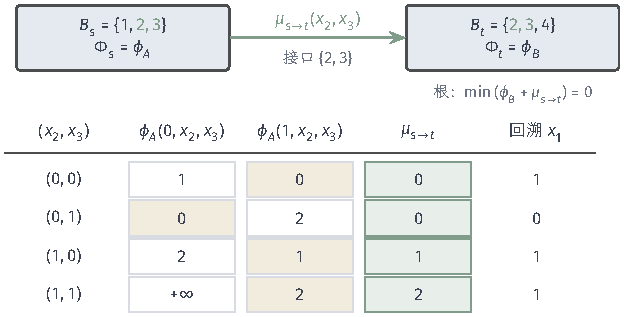
\includegraphics[width=105.650mm]{figures/01-basic-mathematics/04-graphs/tikz/c5-bag-message-table/figure.pdf}
  \caption{两袋之间的消息。左袋$B_s=\{1,2,3\}$只含$\phi_A$，右袋$B_t=\{2,3,4\}$只含$\phi_B$，接口为$\{2,3\}$（绿色）。下方表格对接口的每种取值比较$x_1=0,1$两个候选，取较小者作为消息值，黄色格是被选中的候选；绿色列是消息值，最后一列是回溯表。根袋$B_t$把消息与$\phi_B$相加后对$x_2,x_3,x_4$取最小，得到最优值$0$。}
  \label{fig:graph-dp-bag-message-table}
\end{figure}

选$t$为根，根处合并袋成本与全部入消息，再对根袋的全部变量取最小：
\[
\min_{x_2,x_3,x_4}\bigl[\phi_B(x_2,x_3,x_4)+\mu_{s\to t}(x_2,x_3)\bigr]=0,
\]
在$(x_2,x_3,x_4)=(0,1,0)$处达到，因为$\phi_B(0,1,0)=0$且$\mu_{s\to t}(0,1)=0$，而所有值都非负。一般情形下按后序计算：每个节点收齐子节点的消息后向父节点发送消息，最后在根处合并。

\paragraph{为什么沿袋树计算是正确的}
树上消息的正确性依赖于一件事：删去一条边后，两侧除了接收变量以外没有共同的变量。袋树上，这件事由运行交集保证。删去袋树边$\{s,t\}$后，袋树分成两部分；记$s$一侧全部袋中出现的变量为$V_{s|t}$，$t$一侧为$V_{t|s}$。若某个变量$v$在两侧都出现，从它在$s$侧的某个出现位置到$t$侧的某个出现位置，袋树路径必须经过边$\{s,t\}$，由运行交集，$B_s$与$B_t$都含$v$。所以
\begin{equation}
V_{s|t}\cap V_{t|s}\subseteq S_{s,t},
\label{eq:graph-dp-interface-separation}
\end{equation}
即接口把两侧的变量隔开：固定接口取值后，两侧的其余变量互不重叠，可以分别求最小。

\begin{theorem}[袋消息的含义]
\label{thm:graph-dp-bag-message}
设$(\mathcal T,\{B_t\}_{t\in T})$是原始图的树分解，每个局部函数恰好归入一个包含其作用域的袋。对袋树的边$\{s,t\}$，记$A_{s|t}$为归入$s$一侧各袋的局部函数。则对每个接口取值$\bm x_{S_{s,t}}$，
\[
\mu_{s\to t}(\bm x_{S_{s,t}})=\min_{\bm x_{V_{s|t}\setminus S_{s,t}}}\ \sum_{a\in A_{s|t}}\phi_a(\bm x_{S_a}).
\]
进一步，对任意根节点$\rho$，$\min_{\bm x}F(\bm x)=\min_{\bm x_{B_\rho}}\bigl[\Phi_\rho+\sum_{r\in N(\rho)}\mu_{r\to\rho}\bigr]$。
\end{theorem}

\begin{proof}
对$s$一侧的节点数归纳。设$s$在$t$以外的邻居为$r_1,\ldots,r_k$（叶节点时$k=0$）。删去$s$后，$s$一侧的其余节点分成$r_1,\ldots,r_k$各自的一侧。由式~\eqref{eq:graph-dp-interface-separation}应用于边$\{r_j,s\}$，$V_{r_j|s}$与$B_s$的公共变量都在$S_{r_j,s}$中；不同的$r_j,r_l$两侧若有公共变量，它在袋树上的两个出现位置之间的路径经过$s$，所以也在$B_s$中。因此集合
\[
B_s\setminus S_{s,t},\qquad V_{r_1|s}\setminus B_s,\qquad\ldots,\qquad V_{r_k|s}\setminus B_s
\]
两两不交，它们的并恰为$V_{s|t}\setminus S_{s,t}$。另一方面，$A_{s|t}$按函数归入的节点分为归入$s$的部分和归入各$r_j$一侧的部分$A_{r_j|s}$，每个函数恰在一处；$A_{r_j|s}$中函数的变量都在$V_{r_j|s}$中，其中属于$B_s$的部分又在$S_{r_j,s}$中。

现在固定$\bm x_{B_s}$。各$A_{r_j|s}$中函数之和只依赖$\bm x_{S_{r_j,s}}$与互不相交的变量组$\bm x_{V_{r_j|s}\setminus B_s}$，按式~\eqref{eq:graph-dp-min-rules}后的第三条规则可以分别求最小，由归纳假设，第$j$项的最小值为$\mu_{r_j\to s}(\bm x_{S_{r_j,s}})$。再对$\bm x_{B_s\setminus S_{s,t}}$求最小值，就得到式~\eqref{eq:graph-dp-bag-message}。根处的等式用同样的拆分得到：由顶点覆盖，全部变量是$B_\rho$与各$V_{r|\rho}\setminus B_\rho$的不交并，全部函数分为归入$\rho$的与归入各邻居一侧的。
\end{proof}

证明用到了三项条件：运行交集保证接口隔开两侧；顶点覆盖保证根处的汇总涉及全部变量；每个函数恰好归入一个袋，保证每一项只计一次。少了任何一项，递推得到的数都可能不等于原问题的最小值。

\subsection{配置恢复与计算开销}

\paragraph{沿袋树回溯}
计算$\mu_{s\to t}$时，对每个接口取值同时记录达到最小值的非接口变量取值$\beta_{s\to t}(\bm x_{S_{s,t}})$，即袋上的回溯表。根处取使合并值最小的$\bm x_{B_\rho}$，然后按前序：对已确定全部变量的节点$t$及其子节点$s$，令$\bm x_{B_s\setminus S_{s,t}}=\beta_{s\to t}(\bm x_{S_{s,t}})$。$B_s$中属于接口的变量此前已在$B_t$中取定；不属于接口的变量由运行交集不会出现在$s$一侧以外，因而此前没有被赋值。所以每个变量恰好被赋值一次，在它出现的所有袋中取同一个值。

例子中根取$(x_2,x_3,x_4)=(0,1,0)$，查左袋的回溯表得$\beta_{s\to t}(0,1)=0$，即$x_1=0$。恢复的配置$(0,0,1,0)$代回原始局部函数得$\phi_A(0,0,1)+\phi_B(0,1,0)=0+0=0$，与最优值一致，也与第~\ref{sec:graph-variable-elimination}节两种消元次序的结果相同。若根处的最小值为$+\infty$，则报告没有可行配置。

\paragraph{时间与存储}
设袋树有$N$个节点，宽度为$k$，各变量至多$q$个状态。计算$\mu_{s\to t}$时要枚举$\bm x_{B_s}$的至多$q^{k+1}$种取值，每种取值读取归入$s$的各函数一次、读取$s$的其他入消息各一次，所以全部向上消息的时间约为
\[
\sum_{s}\bigl(|A_s|+|N(s)|\bigr)q^{k+1}=O\bigl((|A|+N)\,q^{k+1}\bigr),
\]
其中$|A_s|$是归入$s$的函数个数，并用到了袋树中$\sum_s|N(s)|=2(N-1)$。每张消息表与回溯表各有$\prod_{i\in S_{s,t}}|\mathcal X_i|\leq q^{k}$项。若还需要每个袋上各取值的最小总成本，就像树上那样再按前序发送一遍反向消息，时间与存储加倍。

这里的计算是精确的，但精确不等于便宜。宽度$k$出现在指数上，$q=10$、$k=10$时一张袋表就有$10^{11}$项；若查询要求保留很多变量的联合最小成本表，输出本身也可能大得不可承受。另外，本节的正确性证明依赖袋树无环和运行交集。若直接在带环的原始图上按式~\eqref{eq:graph-dp-tree-message}反复交换消息，同一部分成本会沿环被重复计入，上面的证明不再适用；这类迭代是否收敛、收敛到什么，需要另外分析，留到后续推断部分。

\subsection{计数与有限加权求和}

\paragraph{换一种组合与汇总}
保持同样的局部结构和袋树，可以回答另外两个问题。第一个问题是：有多少个可行配置？把每个局部函数换成可行性指示$\mathbb I\{\phi_a(\bm x_{S_a})<+\infty\}$，一个配置可行当且仅当这些指示全为$1$，即它们的乘积为$1$；于是可行配置数为$\sum_{\bm x}\prod_a\mathbb I\{\phi_a<+\infty\}$。第二个问题是：给每个局部函数一张非负权重表$w_a(\bm x_{S_a})$，把配置的权重定义为各局部权重之积，求全部配置的权重总和$\sum_{\bm x}\prod_a w_a(\bm x_{S_a})$。两者都把“局部项相加、对变量取最小”换成“局部项相乘、对变量求和”。

推导与最小成本完全平行。式~\eqref{eq:graph-dp-min-rules}中的三条规则换成：有限求和可以分步进行；与求和变量无关的因子可以提到求和号外，即$\sum_y c\,g(y)=c\sum_y g(y)$；互不相交的变量组上，乘积之和等于和之积。于是把式~\eqref{eq:graph-dp-bag-message}中的加号换成乘号、最小化换成求和，消息就变成“$s$一侧的可行配置数”或“$s$一侧的权重总和”，以接口取值为索引。

表~\ref{tab:graph-dp-weights}给出四变量例子的权重表，权重恰在禁止的组合处为$0$。表~\ref{tab:graph-dp-three-aggregations}对接口的每种取值并列三种任务的左袋消息和右袋汇总值，最后一行是根处的结果：最小成本为$0$，可行配置有$10$个，权重总和为$19$。逐一枚举$16$个配置可以核对这三个数。

\begin{table}[!htb]
  \centering
  \caption{四变量例子的非负局部权重。第一列的三位二进制串对$w_A$表示$(x_1,x_2,x_3)$，对$w_B$表示$(x_2,x_3,x_4)$；权重为$0$的位置恰是表~\ref{tab:graph-dp-ternary-tables}中成本为$+\infty$的位置。}
  \label{tab:graph-dp-weights}
  \begin{tabular}{ccccccccc}
    \toprule
    取值 & $000$ & $001$ & $010$ & $011$ & $100$ & $101$ & $110$ & $111$\\
    \midrule
    $w_A$ & $1$ & $2$ & $1$ & $0$ & $2$ & $1$ & $1$ & $1$\\
    $w_B$ & $1$ & $1$ & $2$ & $0$ & $0$ & $2$ & $1$ & $2$\\
    \bottomrule
  \end{tabular}
\end{table}

\begin{table}[!htb]
  \centering
  \caption{三种任务在同一接口上的消息。最小成本使用$\min$与$+$，可行计数与加权总和使用$\sum$与$\times$。“左”列是从$B_s$发出的消息，对$x_1$汇总；“右”列是$B_t$对$x_4$的汇总；根处对每个接口取值组合两列（最小成本相加，其余相乘），再对接口汇总（最小成本取最小，其余求和）。}
  \label{tab:graph-dp-three-aggregations}
  \begin{tabular}{ccccccc}
    \toprule
    & \multicolumn{2}{c}{最小成本} & \multicolumn{2}{c}{可行计数} & \multicolumn{2}{c}{加权总和}\\
    \cmidrule(lr){2-3}\cmidrule(lr){4-5}\cmidrule(lr){6-7}
    $(x_2,x_3)$ & 左 & 右 & 左 & 右 & 左 & 右\\
    \midrule
    $(0,0)$ & $0$ & $1$ & $2$ & $2$ & $3$ & $2$\\
    $(0,1)$ & $0$ & $0$ & $2$ & $1$ & $3$ & $2$\\
    $(1,0)$ & $1$ & $0$ & $2$ & $1$ & $2$ & $2$\\
    $(1,1)$ & $2$ & $1$ & $1$ & $2$ & $1$ & $3$\\
    \midrule
    根处 & \multicolumn{2}{c}{$\min(1,0,1,3)=0$} & \multicolumn{2}{c}{$4+2+2+2=10$} & \multicolumn{2}{c}{$6+6+4+3=19$}\\
    \bottomrule
  \end{tabular}
\end{table}

三种任务的输出含义不同。最小成本是一个配置的值，还可以回溯出达到它的配置；计数和加权总和是对全部配置的汇总，没有“达到它的配置”可言。例如接口取$(1,1)$时，左袋的最小成本消息为$2$，计数消息为$1$，因为$x_1=0$的那一行被禁止，只剩$x_1=1$一个可行选择；加权消息为$0+1=1$。

\paragraph{半环与分配律}
上面三种任务共用同一套递推，是因为它们的运算满足同样的代数规则。设集合$\mathcal S$上有两种运算：$\oplus$用于跨不同取值的汇总，$\otimes$用于在一个配置内组合各局部项。若两种运算都满足结合律和交换律，各有单位元$\bar0$与$\bar1$，满足$\bar0\otimes a=\bar0$，并且$\otimes$对$\oplus$满足分配律
\[
a\otimes(b\oplus c)=(a\otimes b)\oplus(a\otimes c),
\]
就称$(\mathcal S,\allowbreak\oplus,\allowbreak\otimes,\allowbreak\bar0,\allowbreak\bar1)$为交换\term{半环}（semiring）。最小成本对应$(\mathbb R\cup\{+\infty\},\allowbreak\min,\allowbreak+,\allowbreak+\infty,\allowbreak0)$，此时分配律就是$a+\min(b,c)=\min(a+b,a+c)$；计数对应自然数上的$(+,\times,0,1)$；加权求和对应非负实数上的$(+,\times,0,1)$；只判断是否存在可行配置时，还可以用布尔值上的“或”与“且”。把变量消元和袋消息中的$\min$换成$\oplus$、$+$换成$\otimes$，前面的正确性证明逐字成立，因为证明只用到了结合律、交换律和分配律。半环不要求减法或除法。

\paragraph{不能随意交换的汇总}
分配律只保证同一种汇总可以分步、移项。若一个问题对一部分变量取最大值、对另一部分变量求和，两种汇总一般不能交换次序。例如对表$h(x,y)$，$h(0,0)=h(1,1)=4$、$h(0,1)=h(1,0)=0$，有
\[
\max_x\sum_y h(x,y)=4,\qquad \sum_y\max_x h(x,y)=8 .
\]
前者要求所有$y$共用同一个$x$，后者允许$x$随$y$改变。这类混合问题只能按限定的次序消元，所需的中间表可能比单一汇总时大。把非负权重归一化为概率还要求总和为正且有限；这些概率解释、边缘化查询以及带环图上的近似消息方法，都留到后续推断部分。

% 第5章第7节：本章小结。

\section{本章小结}
\label{sec:graph-dp-summary}

本章处理的问题由局部函数组成：每个变量取有限个状态，整体成本是若干局部项之和，每一项只读取少数变量。计算的核心始终是同一个动作：固定一组接口变量，把只在一侧出现的变量汇总掉，留下一张以接口为索引的表。链上，接口是一个变量，表沿链逐个传递；树上，接口仍是一个变量，但一个顶点要合并多棵子树传来的消息；一般依赖图上，变量消元按任意次序逐个汇总变量，正确性不变，中间表的作用域却随次序变化。树分解把这些同时处理的变量组织成袋树，消元次序可以机械地产生树分解，弦图上还能用极大团和最大权生成树得到团树；最后，袋上的消息把树上的递推推广到一般图。

这些步骤中有三种不能互相替代的对象。局部函数表记录数值，决定消息的具体取值；原始图记录哪些变量共同出现，决定消元时的填充边和袋必须容纳的团；袋树记录计算的组织方式，决定消息沿什么路径传递、以什么为索引。原始图不能恢复函数表，袋树的边也不是原始图的边；混淆它们会导致把高阶约束错拆成成对规则，或在袋之间重复累计成本。

精确计算依赖一组明确的条件：局部函数给出完整的作用域；状态集合有限；组合与汇总的运算满足结合律、交换律与分配律，即构成半环；每个局部函数恰好归入一个包含其作用域的袋；袋树满足运行交集，使接口把两侧的变量隔开。计算规模则主要由袋的大小控制，宽度为$k$、每个变量至多$q$个状态时，袋表至多$q^{k+1}$项。树宽小的图上精确计算可行，树宽大的图上同样的方法仍然正确，但可能无法承受。后续的概率模型会把这些表解释为未归一化的概率、把求和解释为边缘化，但归一化条件、查询中不同汇总的次序以及带环图上的近似方法，都需要在那里另外说明，不能由本章的结论直接推出。

本章比较的是有限配置：每个变量取离散的状态，目标是在所有配置中找最小值或求汇总。下一章转向另一类任务：顶点上的数值已经给定，要研究它们沿边怎样变化，怎样通过图上的线性算子对它们进行变换和滤波，并据此划分图。所需的工具也随之改变，从有限比较与递推转向内积、二次型和第三部分的谱分解。

